\nonstopmode
\documentclass[aspectratio=169,xcolor={svgnames}]{beamer}
\usepackage[utf8]{inputenc}
% \usepackage[frenchb]{babel}
\usepackage{amsmath}
\usepackage{mathtools}
\usepackage{breqn}
\usepackage{multirow}
\usetheme{boxes}
\usepackage{graphicx}
\usepackage{import}
\usepackage{adjustbox}
\usepackage[absolute,overlay]{textpos}
%\useoutertheme[footline=authortitle,subsection=false]{miniframes}
%\useoutertheme[footline=authorinstitute,subsection=false]{miniframes}
\useoutertheme{infolines}
\setbeamertemplate{headline}{}

\beamertemplatenavigationsymbolsempty

\definecolor{TitleOrange}{RGB}{255,137,0}
\setbeamercolor{title}{fg=TitleOrange}
\setbeamercolor{frametitle}{fg=TitleOrange}

\definecolor{ListOrange}{RGB}{255,145,5}
\setbeamertemplate{itemize item}{\color{ListOrange}$\blacktriangleright$}

\definecolor{verygrey}{RGB}{70,70,70}
\setbeamercolor{normal text}{fg=verygrey}


\usepackage{tabu}
\usepackage{multicol}
\usepackage{vwcol}
\usepackage{stmaryrd}
\usepackage{graphicx}

\usepackage[normalem]{ulem}

\AtBeginSection[]{
  \begin{frame}
  \vfill
  \centering
  \begin{beamercolorbox}[sep=8pt,center,shadow=true,rounded=true]{title}
    \usebeamerfont{title}\insertsectionhead\par%
  \end{beamercolorbox}
  \vfill
  \end{frame}
}

\title{Garage, the low-tech storage platform for geo-distributed clusters}
\author{Alex Auvolat, Deuxfleurs}
\date{FOSDEM'24, 2024-02-03}

\begin{document}

\begin{frame}
	\centering
	
\includegraphics[width=.3\linewidth]{../../sticker/Garage.png}
	\vspace{1em}

	{\large\bf Alex Auvolat, Deuxfleurs Association}
	\vspace{1em}

	\url{https://garagehq.deuxfleurs.fr/}

	Matrix channel: \texttt{\#garage:deuxfleurs.fr}
\end{frame}

\begin{frame}
	\frametitle{Who I am}
	\begin{columns}[t]
		\begin{column}{.2\textwidth}
			\centering
			\adjincludegraphics[width=.4\linewidth, valign=t]{../assets/alex.jpg}
		\end{column}
		\begin{column}{.6\textwidth}
			\textbf{Alex Auvolat}\\
			PhD; co-founder of Deuxfleurs
		\end{column}
		\begin{column}{.2\textwidth}
			~
		\end{column}
	\end{columns}
	\vspace{2em}

	\begin{columns}[t]
		\begin{column}{.2\textwidth}
			\centering
			\adjincludegraphics[width=.5\linewidth, valign=t]{../assets/logos/deuxfleurs.pdf}
		\end{column}
		\begin{column}{.6\textwidth}
			\textbf{Deuxfleurs}\\
			A non-profit self-hosting collective,\\
			member of the CHATONS network
		\end{column}
		\begin{column}{.2\textwidth}
			\centering
			\adjincludegraphics[width=.7\linewidth, valign=t]{../assets/logos/logo_chatons.png}
		\end{column}
	\end{columns}

\end{frame}

\begin{frame}
	\frametitle{Our objective at Deuxfleurs}
	
	\begin{center}
		\textbf{Promote self-hosting and small-scale hosting\\
			as an alternative to large cloud providers}
	\end{center}
	\vspace{2em}
	\visible<2->{
		Why is it hard?
	}
	\visible<3->{
		\vspace{2em}
		\begin{center}
			\textbf{\underline{Resilience}}\\
			{\footnotesize we want good uptime/availability with low supervision}
		\end{center}
	}
\end{frame}

\begin{frame}
	\frametitle{Building a resilient system with cheap stuff}

	\only<1,4-7>{
		\begin{itemize}
			\item \textcolor<5->{gray}{Commodity hardware (e.g. old desktop PCs)\\
				\vspace{.5em}
				\visible<4->{{\footnotesize (can die at any time)}}}
				\vspace{1.5em}
			\item<5-> \textcolor<7->{gray}{Regular Internet (e.g. FTTB, FTTH) and power grid connections\\
				\vspace{.5em}
				\visible<6->{{\footnotesize (can be unavailable randomly)}}}
				\vspace{1.5em}
			\item<7-> \textbf{Geographical redundancy} (multi-site replication)
		\end{itemize}
	}
	\only<2>{
		\begin{center}
			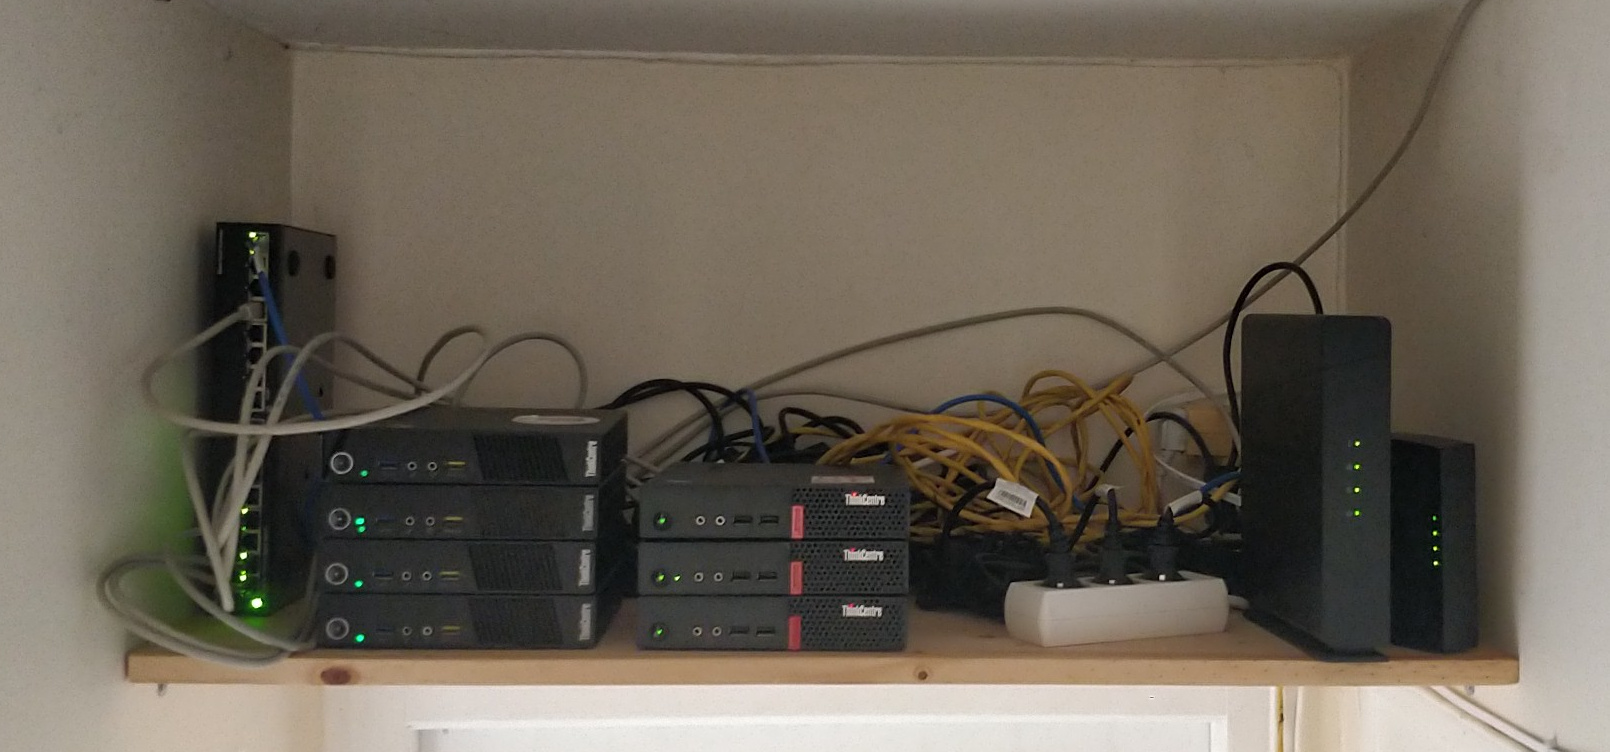
\includegraphics[width=.8\linewidth]{../assets/neptune.jpg}
		\end{center}
	}
	\only<3>{
		\begin{center}
			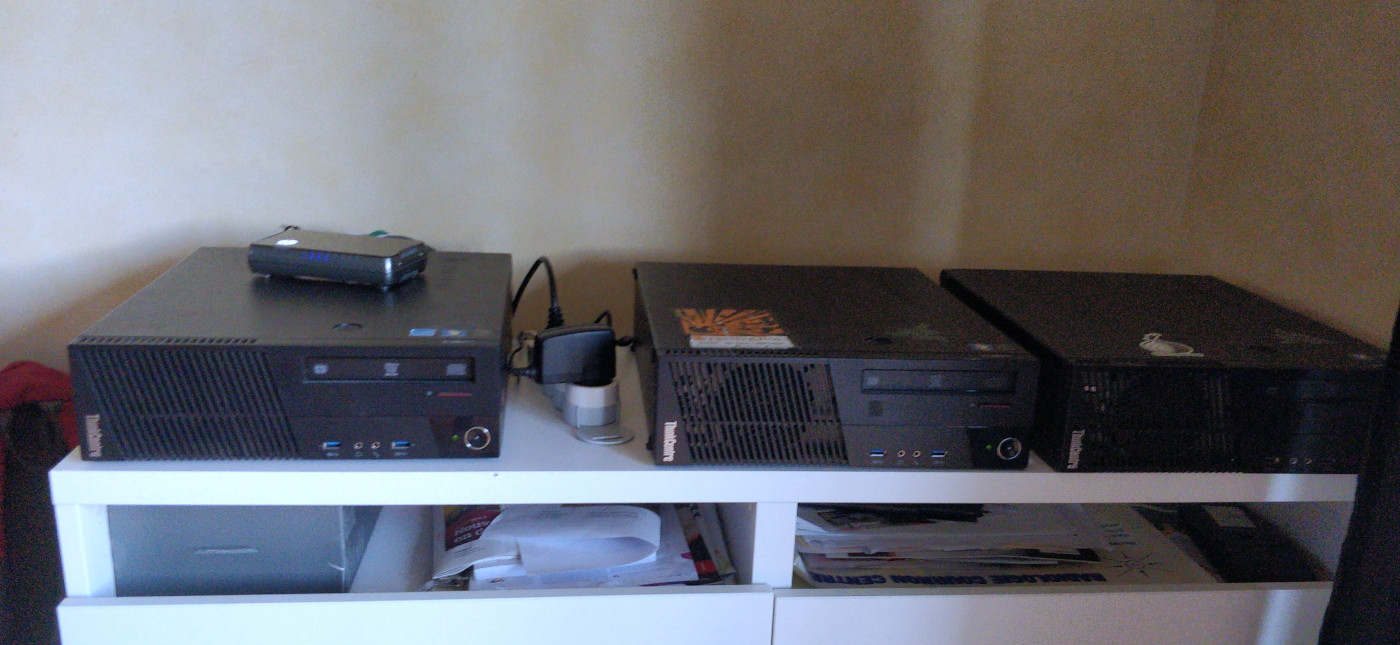
\includegraphics[width=.8\linewidth]{../assets/atuin.jpg}
		\end{center}
	}
	\only<8>{
		\begin{center}
			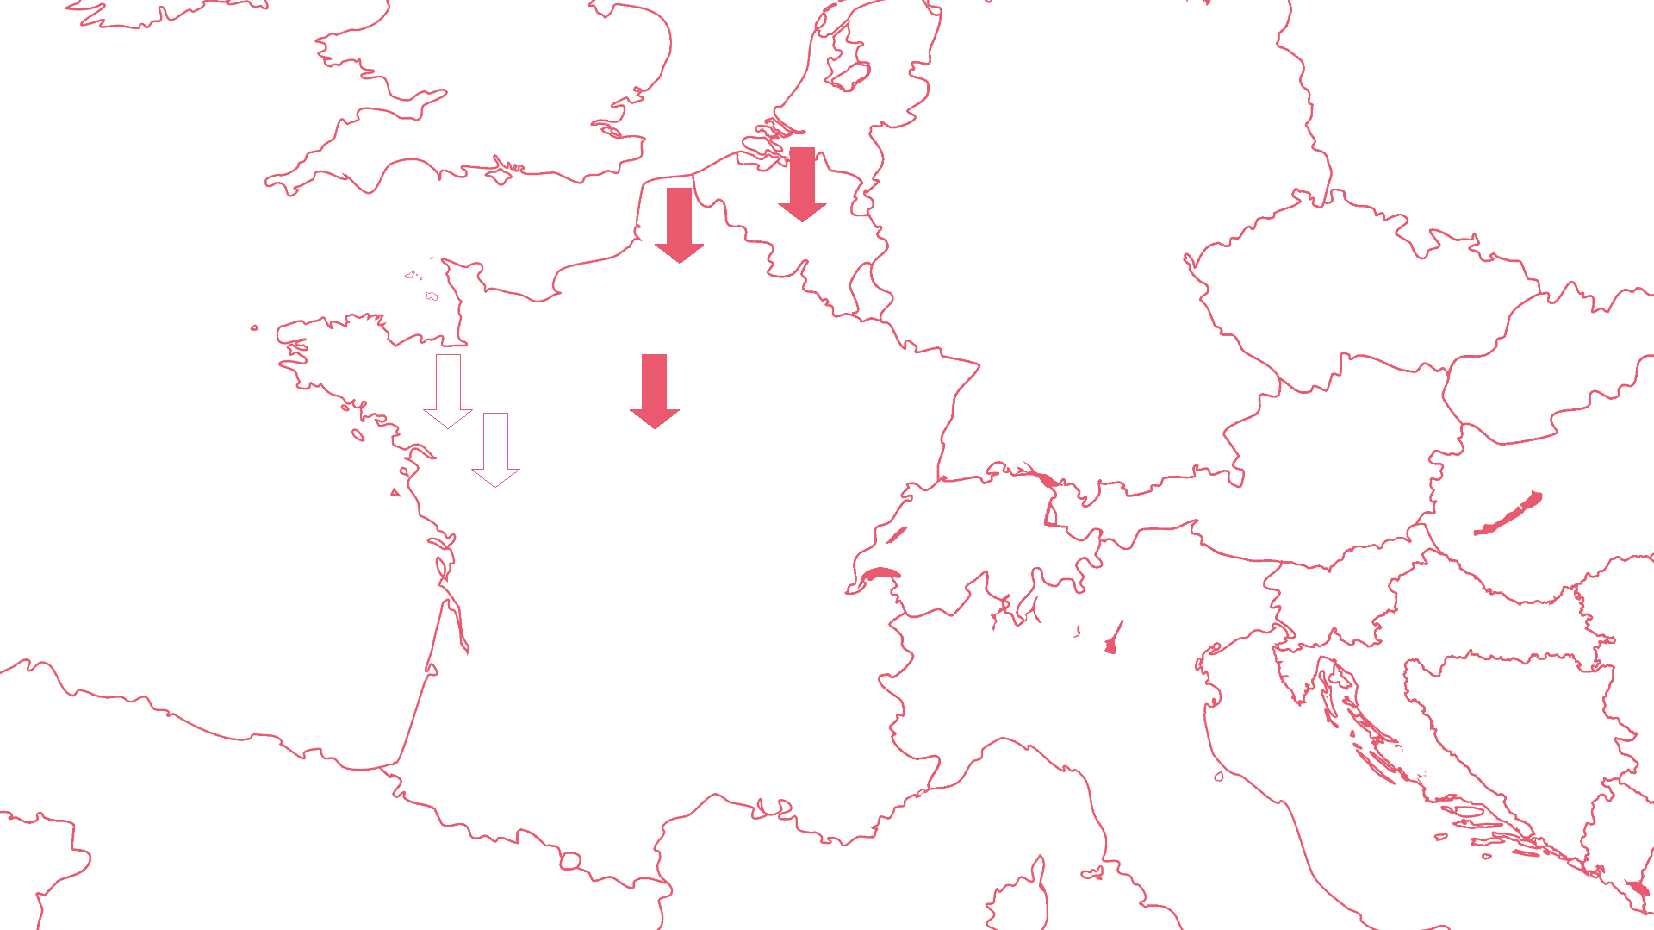
\includegraphics[width=.8\linewidth]{../assets/inframap_jdll2023.pdf}
		\end{center}
	}
\end{frame}

\begin{frame}
	\frametitle{Object storage: a crucial component}
		\begin{center}
			
\includegraphics[height=6em]{../assets/logos/Amazon-S3.jpg}
			\hspace{3em}
			\visible<2->{
\includegraphics[height=5em]{../assets/logos/minio.png}}
			\hspace{3em}
			\visible<3>{
\includegraphics[height=6em]{../../logo/garage_hires_crop.png}}
		\end{center}
		\vspace{1em}
	S3: a de-facto standard, many compatible applications

	\vspace{1em}
	\visible<2->{MinIO is self-hostable but not suited for geo-distributed deployments}

	\vspace{1em}
	\visible<3->{\textbf{Garage is a self-hosted drop-in replacement for the Amazon S3 object store}}
\end{frame}

\begin{frame}
	\frametitle{CRDTs / weak consistency instead of consensus}

	\underline{Internally, Garage uses only CRDTs} (conflict-free replicated data types)

	\vspace{2em}
	No Raft, ... Why?

	\vspace{1em}
	\begin{itemize}
		\item<2-> \textbf{Software complexity}
			\vspace{1em}
		\item<3-> \textbf{Performance issues:}
			\vspace{.5em}
			\begin{itemize}
				\item<4-> The leader is a \textbf{bottleneck} for all requests\\
					\vspace{.5em}
				\item<5-> \textbf{Sensitive to higher latency} between nodes
					\vspace{.5em}
				\item<6-> \textbf{Takes time to reconverge} when disrupted (e.g. node going down)
			\end{itemize}
	\end{itemize}
\end{frame}

\begin{frame}
	\frametitle{The data model of object storage}
	Object storage is basically a \textbf{key-value store}:
	\vspace{.5em}

	{\scriptsize
		\begin{center}
		\begin{tabular}{|l|p{7cm}|}
			\hline
			\textbf{Key: file path + name} & \textbf{Value: file data + metadata} \\
			\hline
			\hline
			\texttt{index.html} &
				\texttt{Content-Type: text/html; charset=utf-8} \newline
				\texttt{Content-Length: 24929} \newline
				\texttt{<binary blob>} \\ 
			\hline
			\texttt{img/logo.svg} &
				\texttt{Content-Type: text/svg+xml} \newline
				\texttt{Content-Length: 13429} \newline
				\texttt{<binary blob>} \\ 
			\hline
			\texttt{download/index.html} &
				\texttt{Content-Type: text/html; charset=utf-8} \newline
				\texttt{Content-Length: 26563} \newline
				\texttt{<binary blob>} \\ 
			\hline
		\end{tabular}
		\end{center}
		}

	\vspace{1em}
	\begin{itemize}
		\item<2> Maps well to CRDT data types
	\end{itemize}
\end{frame}

\begin{frame}
	\frametitle{Performance gains in practice}
	\begin{center}
		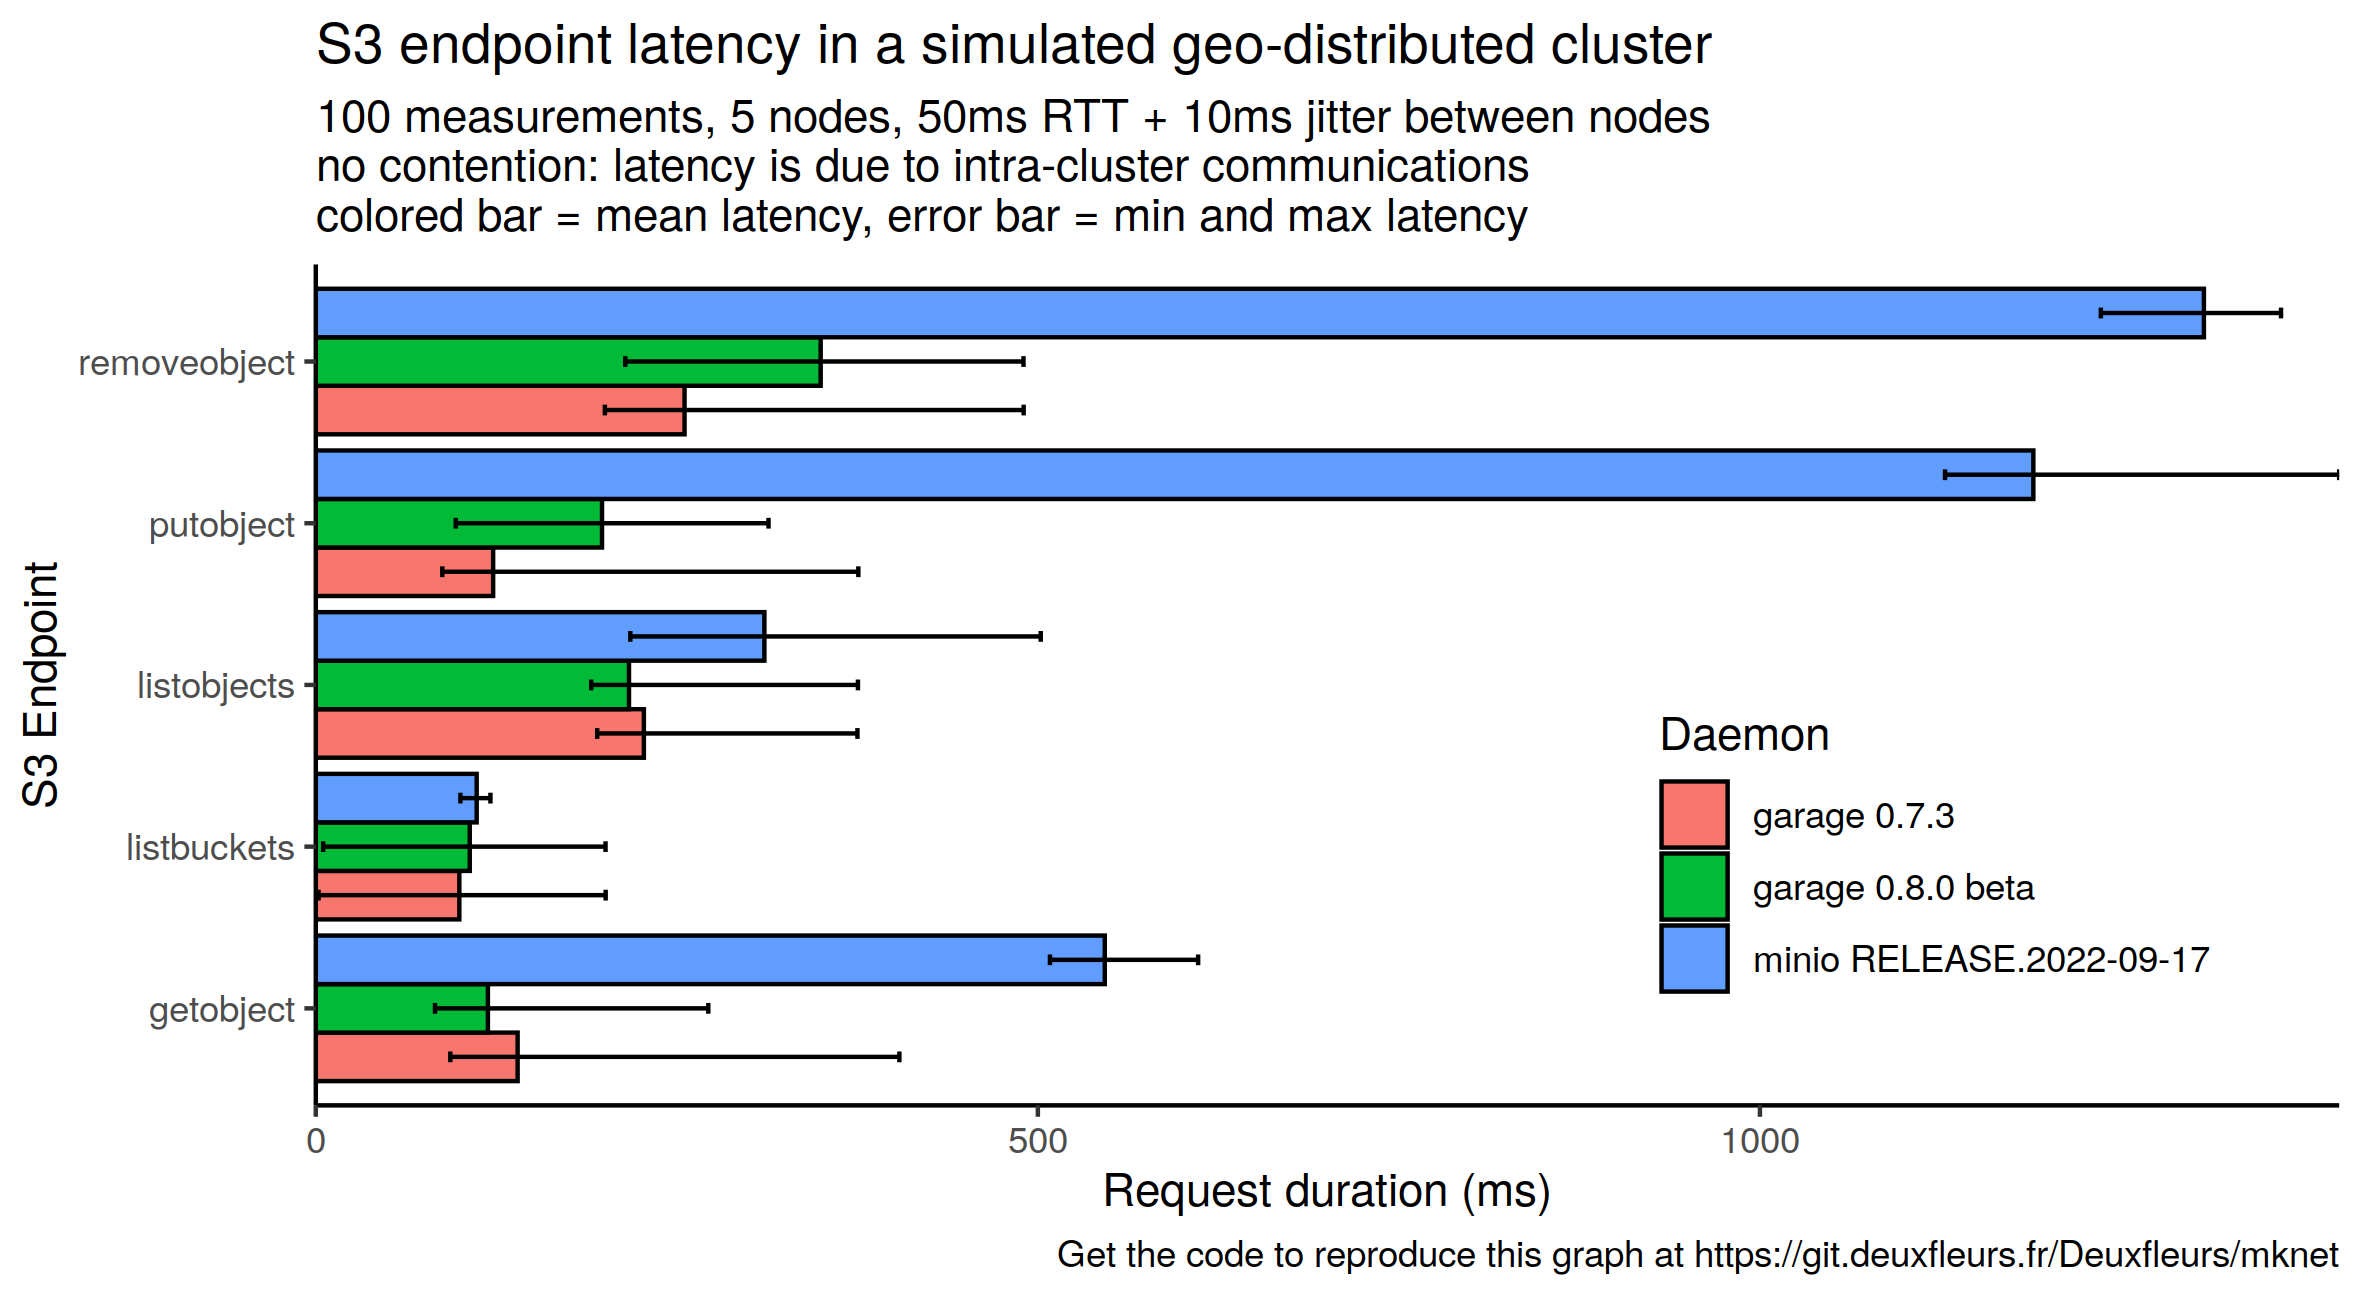
\includegraphics[width=.8\linewidth]{../assets/perf/endpoint_latency_0.7_0.8_minio.png}
	\end{center}
\end{frame}


% ======================================== TIMELINE
% ======================================== TIMELINE
% ======================================== TIMELINE

\section{Recent developments}

% ====================== v0.7.0 ===============================

\begin{frame}
	\begin{center}
		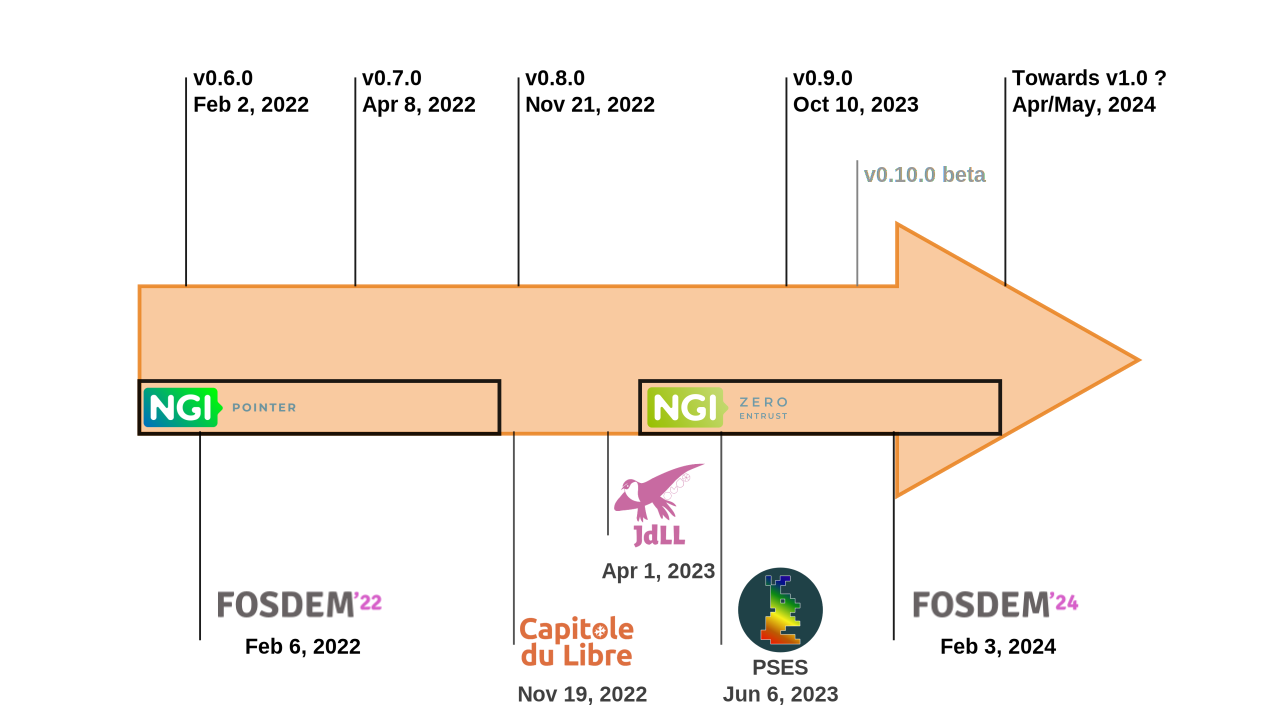
\includegraphics[width=.8\linewidth]{../assets/timeline-22-24.pdf}
	\end{center}
\end{frame}

\begin{frame}
	\frametitle{April 2022 - Garage v0.7.0}
	Focus on \underline{observability and ecosystem integration}
	\vspace{2em}
	\begin{itemize}
		\item \textbf{Monitoring:} metrics and traces, using OpenTelemetry
			\vspace{1em}
		\item Replication modes with 1 or 2 copies / weaker consistency
			\vspace{1em}
		\item Kubernetes integration for node discovery
			\vspace{1em}
		\item Admin API (v0.7.2)
	\end{itemize}
\end{frame}

\begin{frame}
	\frametitle{Metrics (Prometheus + Grafana)}
	\begin{center}
		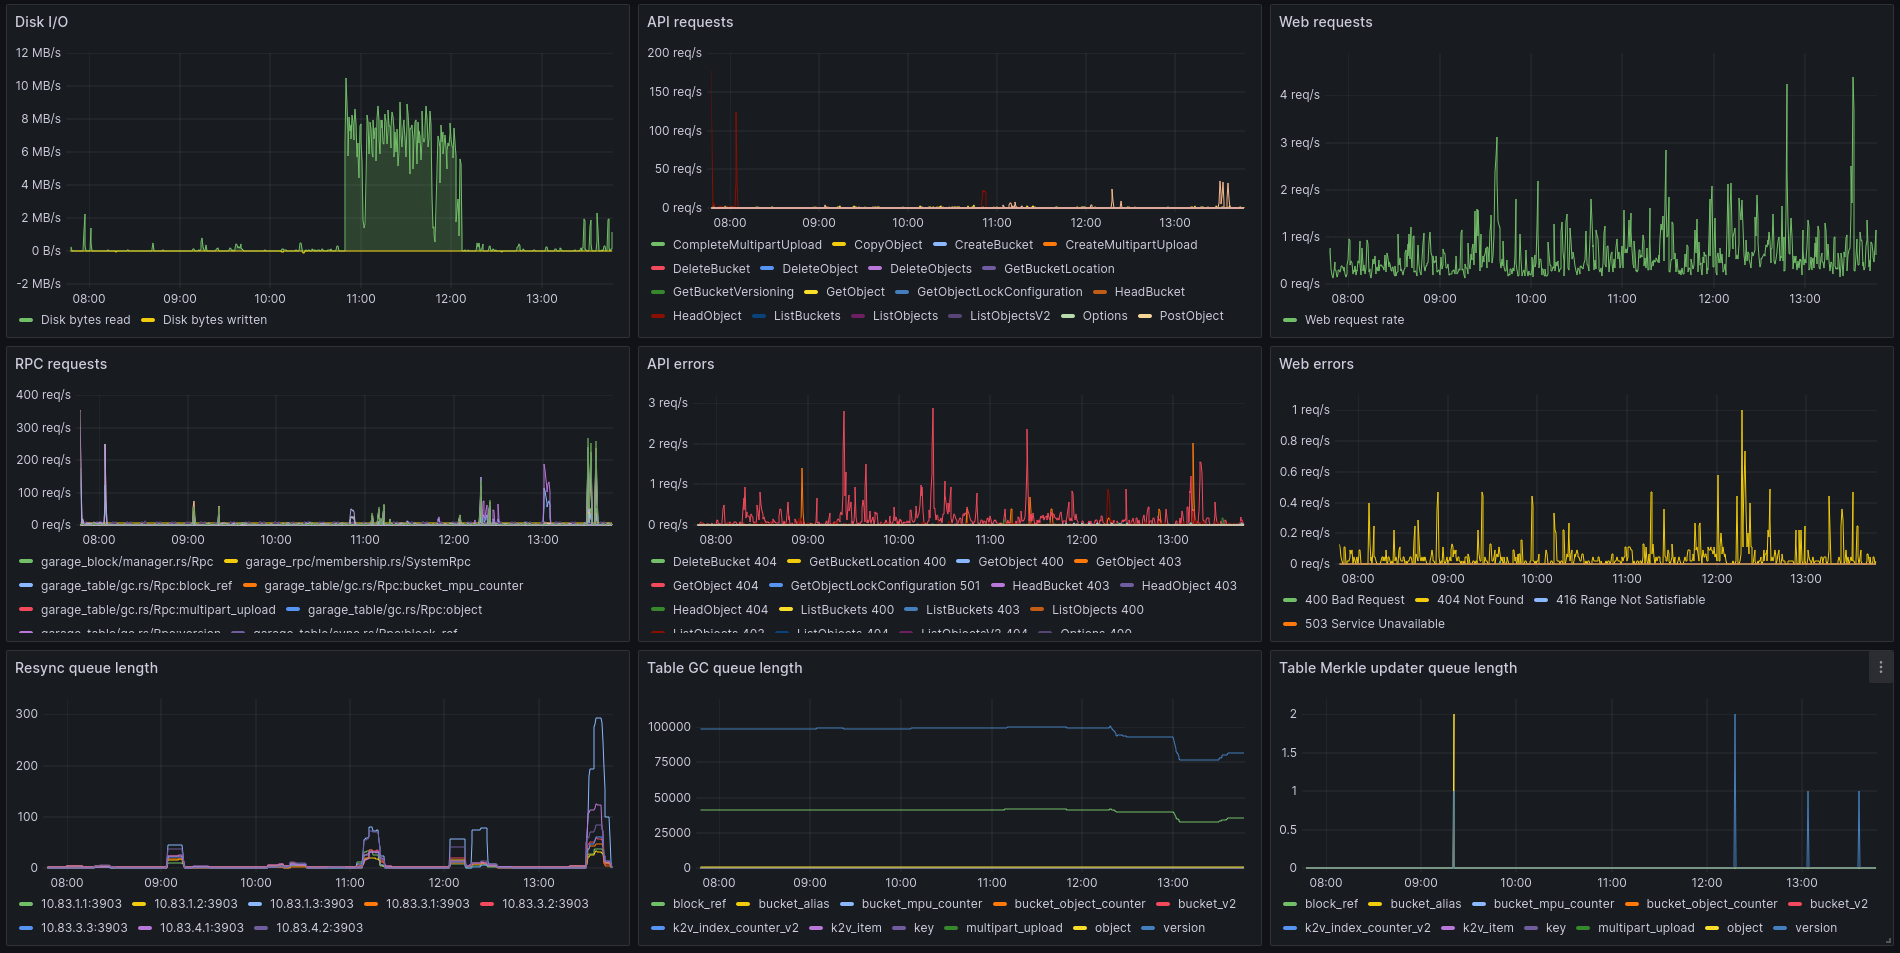
\includegraphics[width=.9\linewidth]{../assets/screenshots/grafana_dashboard.png}
	\end{center}
\end{frame}

\begin{frame}
	\frametitle{Traces (Jaeger)}
	\begin{center}
		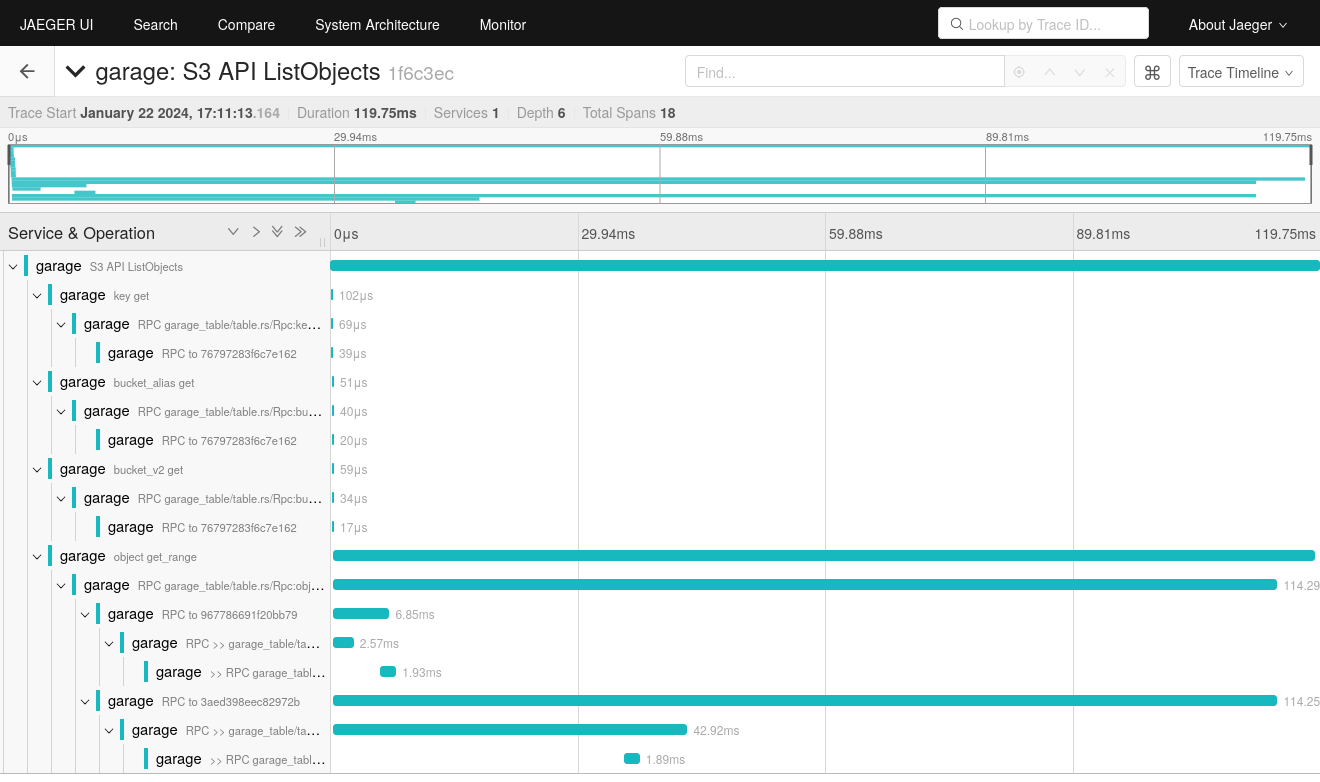
\includegraphics[width=.8\linewidth]{../assets/screenshots/jaeger_listobjects.png}
	\end{center}
\end{frame}

% ====================== v0.8.0 ===============================

\begin{frame}
	\begin{center}
		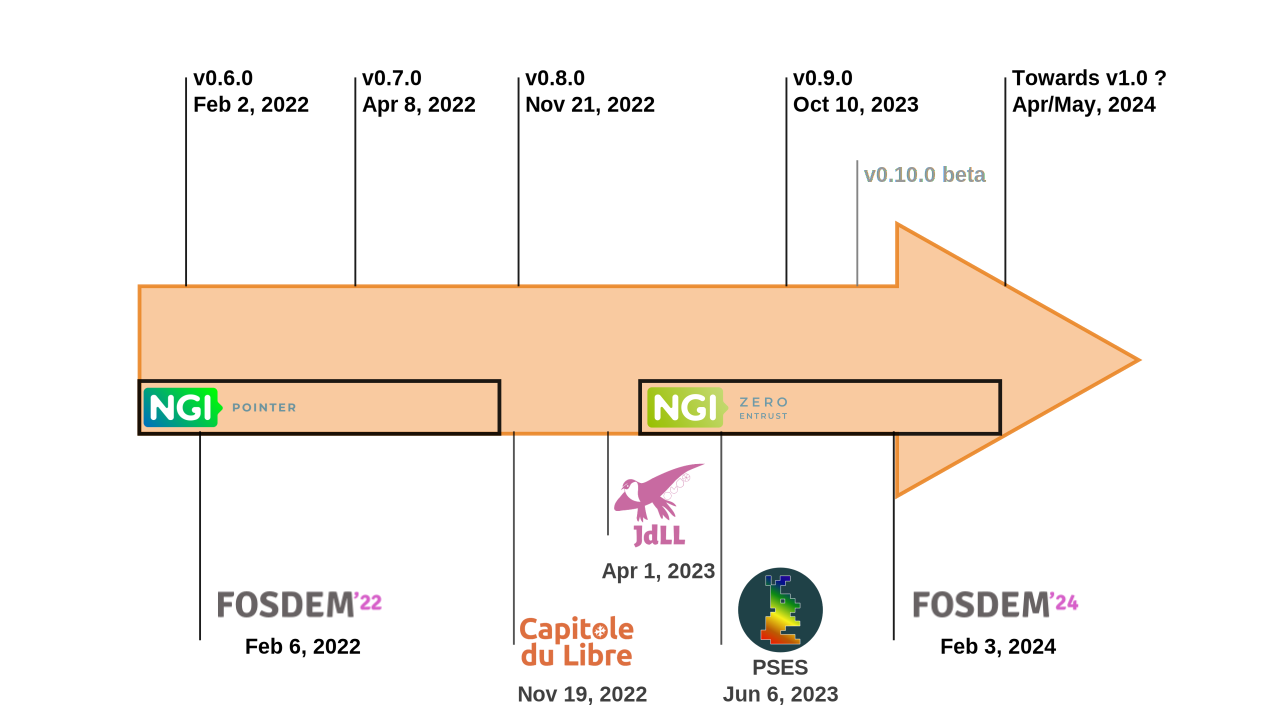
\includegraphics[width=.8\linewidth]{../assets/timeline-22-24.pdf}
	\end{center}
\end{frame}

\begin{frame}
	\frametitle{November 2022 - Garage v0.8.0}
	Focus on \underline{performance}
	\vspace{2em}
	\begin{itemize}
		\item \textbf{Alternative metadata DB engines} (LMDB, Sqlite)
			\vspace{1em}
		\item \textbf{Performance improvements:} block streaming, various optimizations...
			\vspace{1em}
		\item Bucket quotas (max size, max \#objects)
			\vspace{1em}
		\item Quality of life improvements, observability, etc.
	\end{itemize}
\end{frame}

\begin{frame}
	\frametitle{About metadata DB engines}
	\textbf{Issues with Sled:}
	\vspace{1em}
	\begin{itemize}
		\item Huge files on disk
			\vspace{.5em}
		\item Unpredictable performance, especially on HDD
			\vspace{.5em}
		\item API limitations
			\vspace{.5em}
		\item Not actively maintained
	\end{itemize}

	\vspace{2em}
	\textbf{LMDB:} very stable, good performance, file size is reasonable\\
	\textbf{Sqlite} also available as a second choice

	\vspace{1em}
	Sled will be removed in Garage v1.0
\end{frame}

\begin{frame}
	\frametitle{DB engine performance comparison}
	\begin{center}
		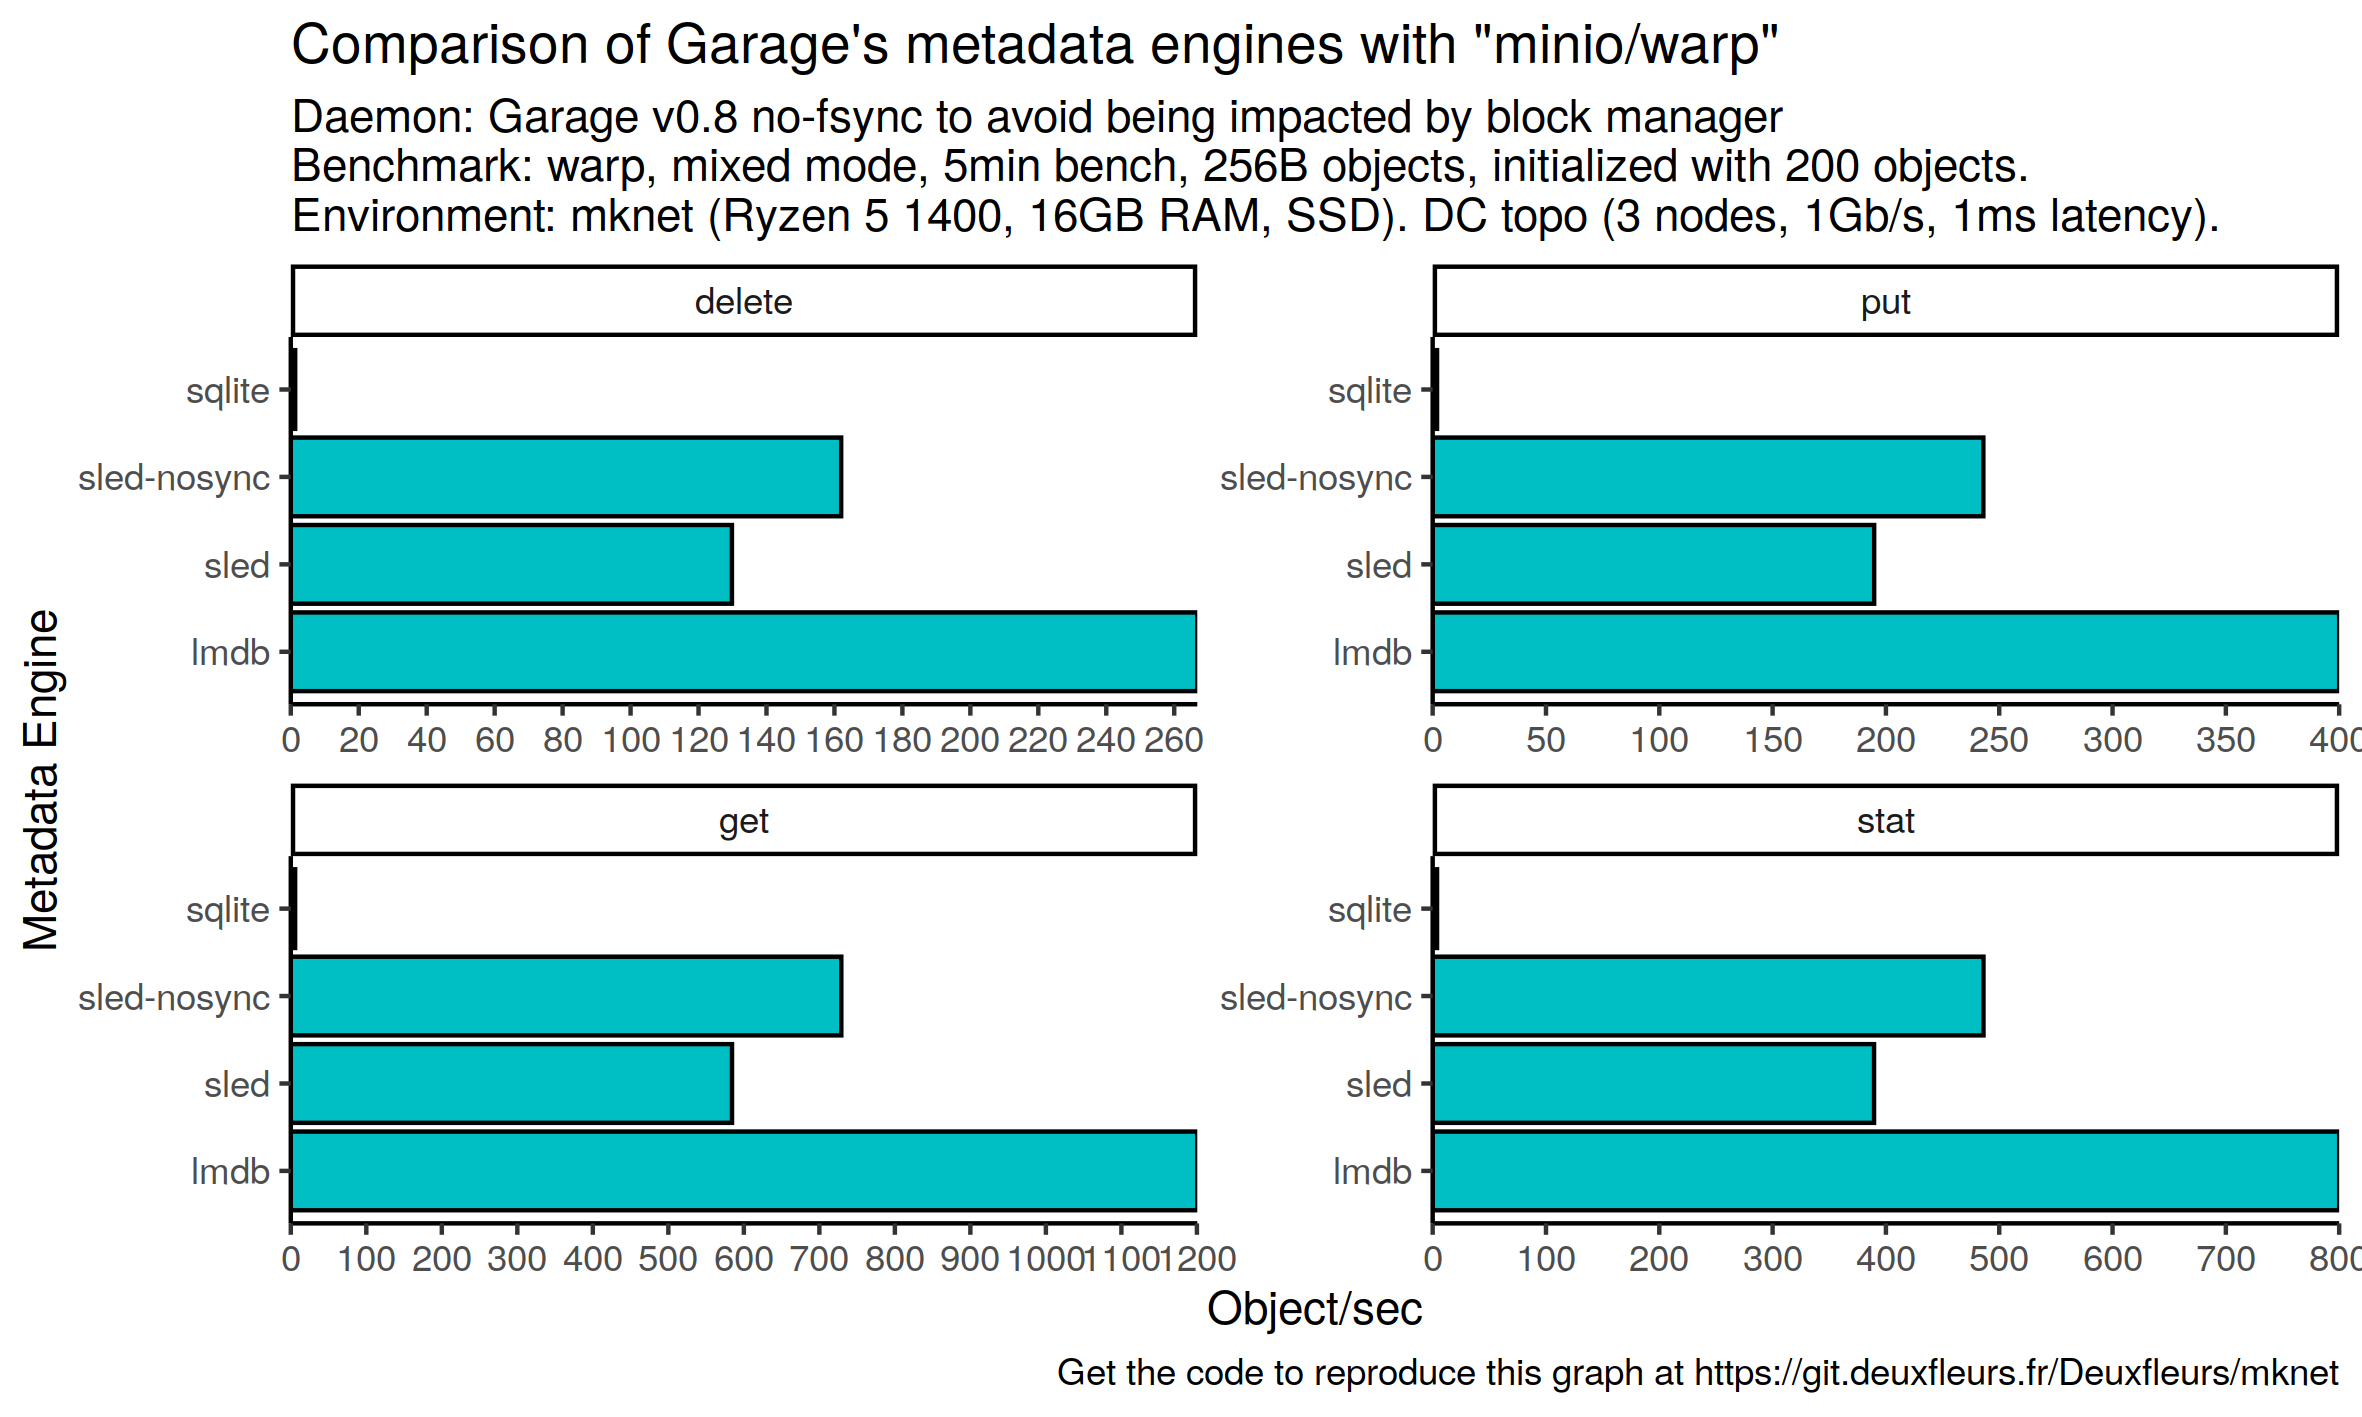
\includegraphics[width=.6\linewidth]{../assets/perf/db_engine.png}
	\end{center}
	NB: Sqlite was slow due to synchronous mode, now configurable
\end{frame}

\begin{frame}
	\frametitle{Block streaming}
	\begin{center}
		\only<1>{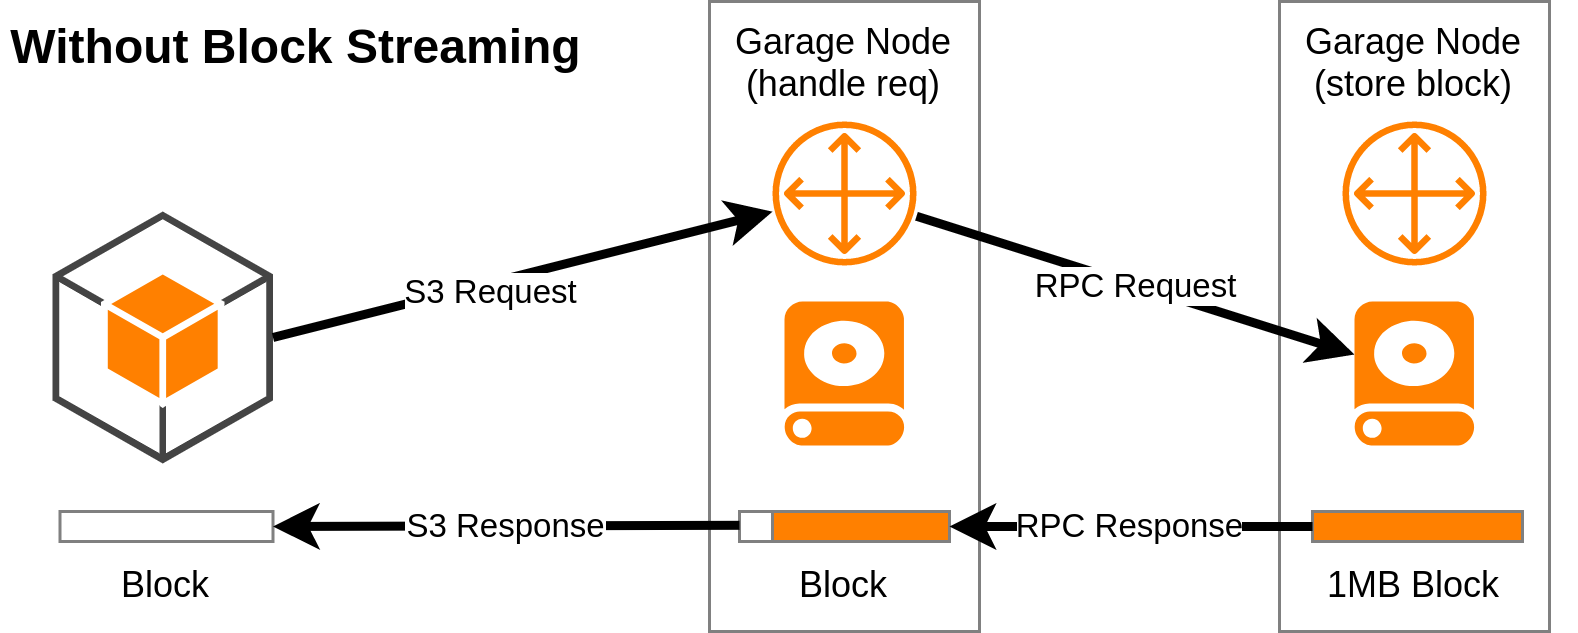
\includegraphics[width=.8\linewidth]{../assets/schema-streaming-1.png}}
		\only<2>{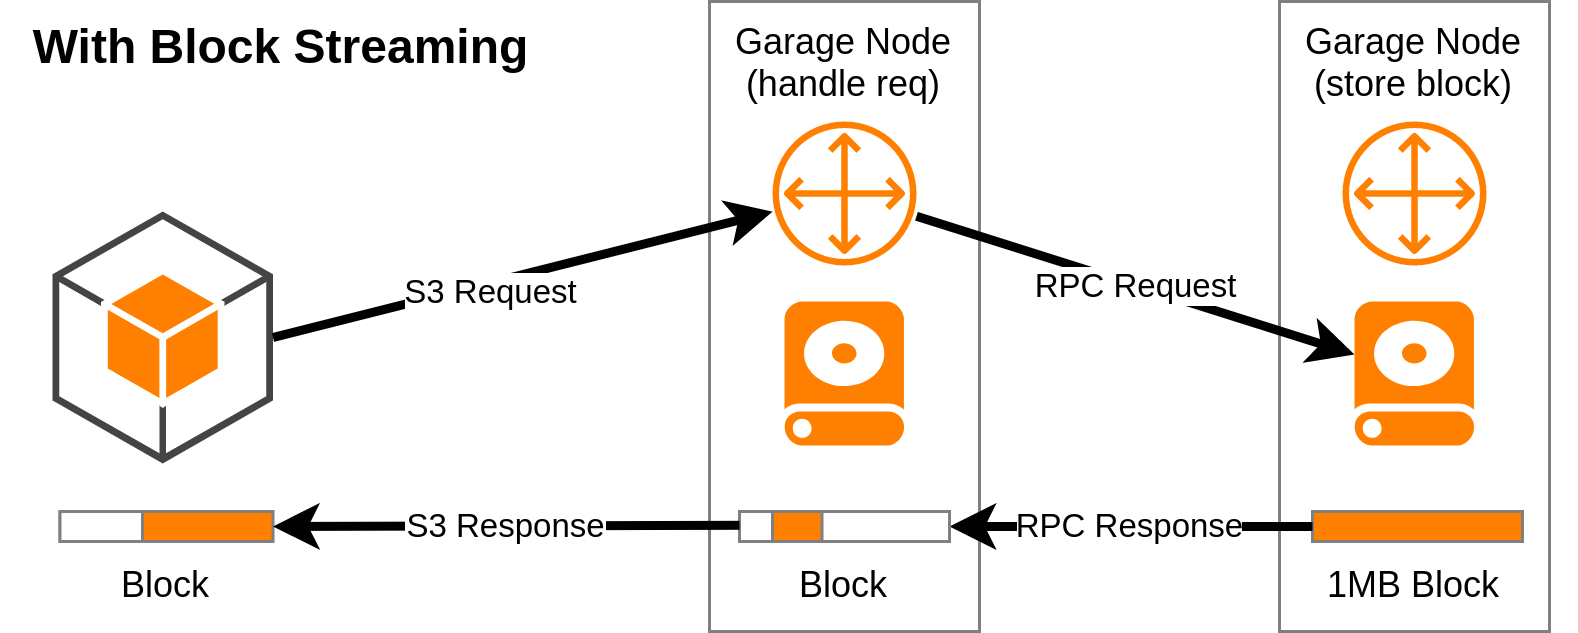
\includegraphics[width=.8\linewidth]{../assets/schema-streaming-2.png}}
	\end{center}
\end{frame}

\begin{frame}
	\frametitle{TTFB benchmark}
	\begin{center}
		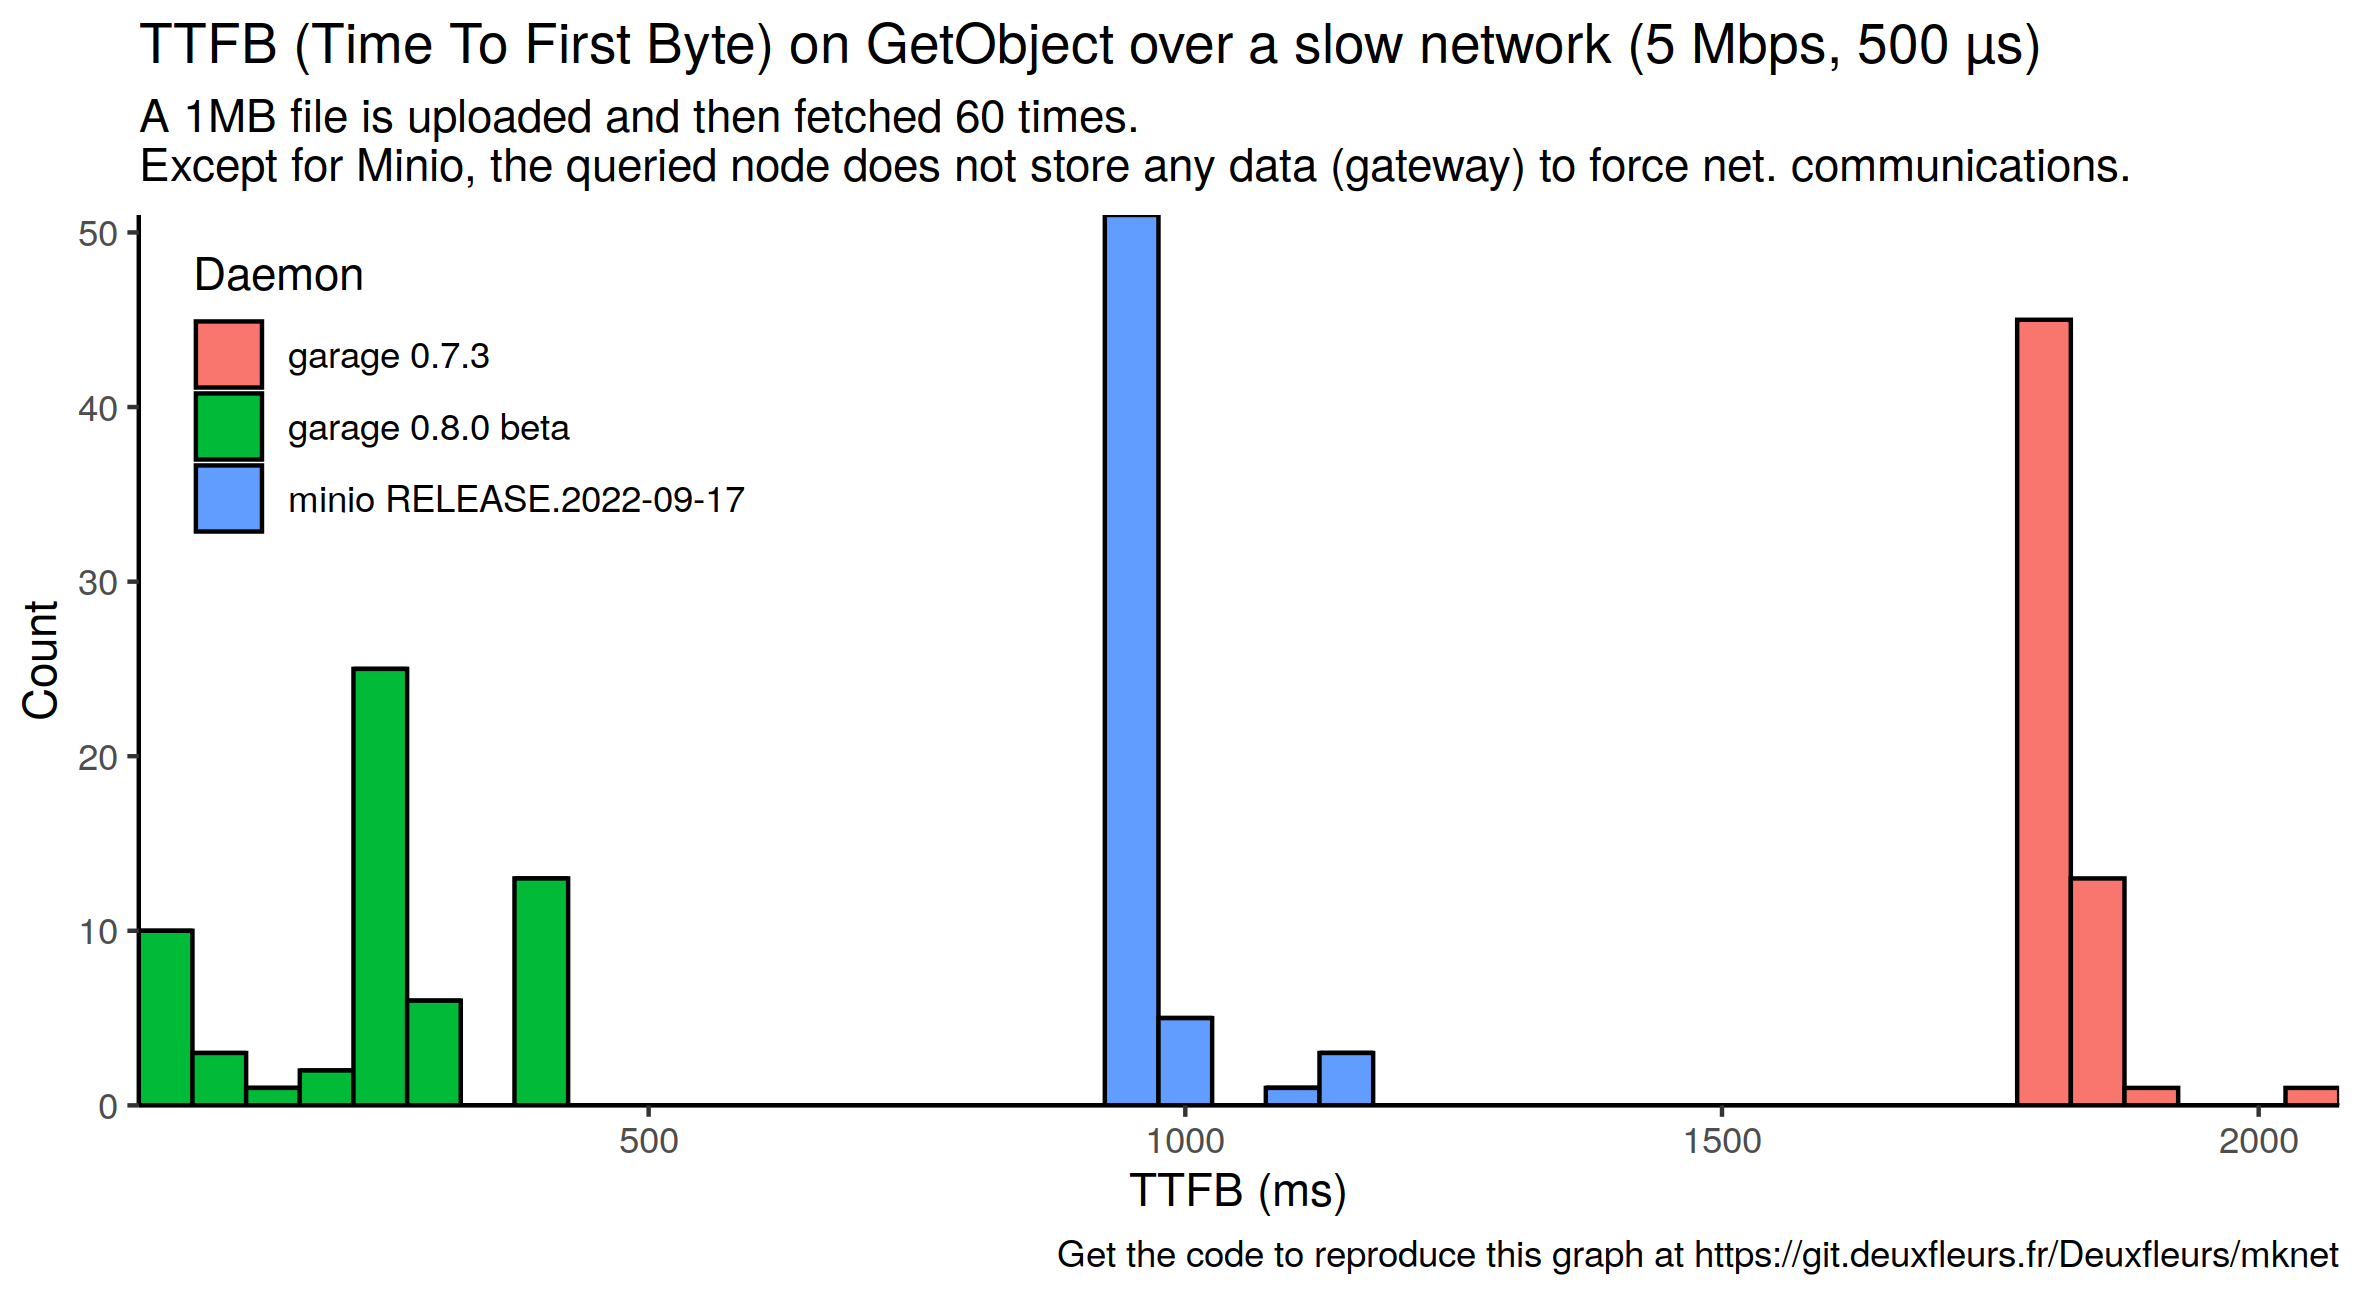
\includegraphics[width=.8\linewidth]{../assets/perf/ttfb.png}
	\end{center}
\end{frame}

\begin{frame}
	\frametitle{Throughput benchmark}
	\begin{center}
		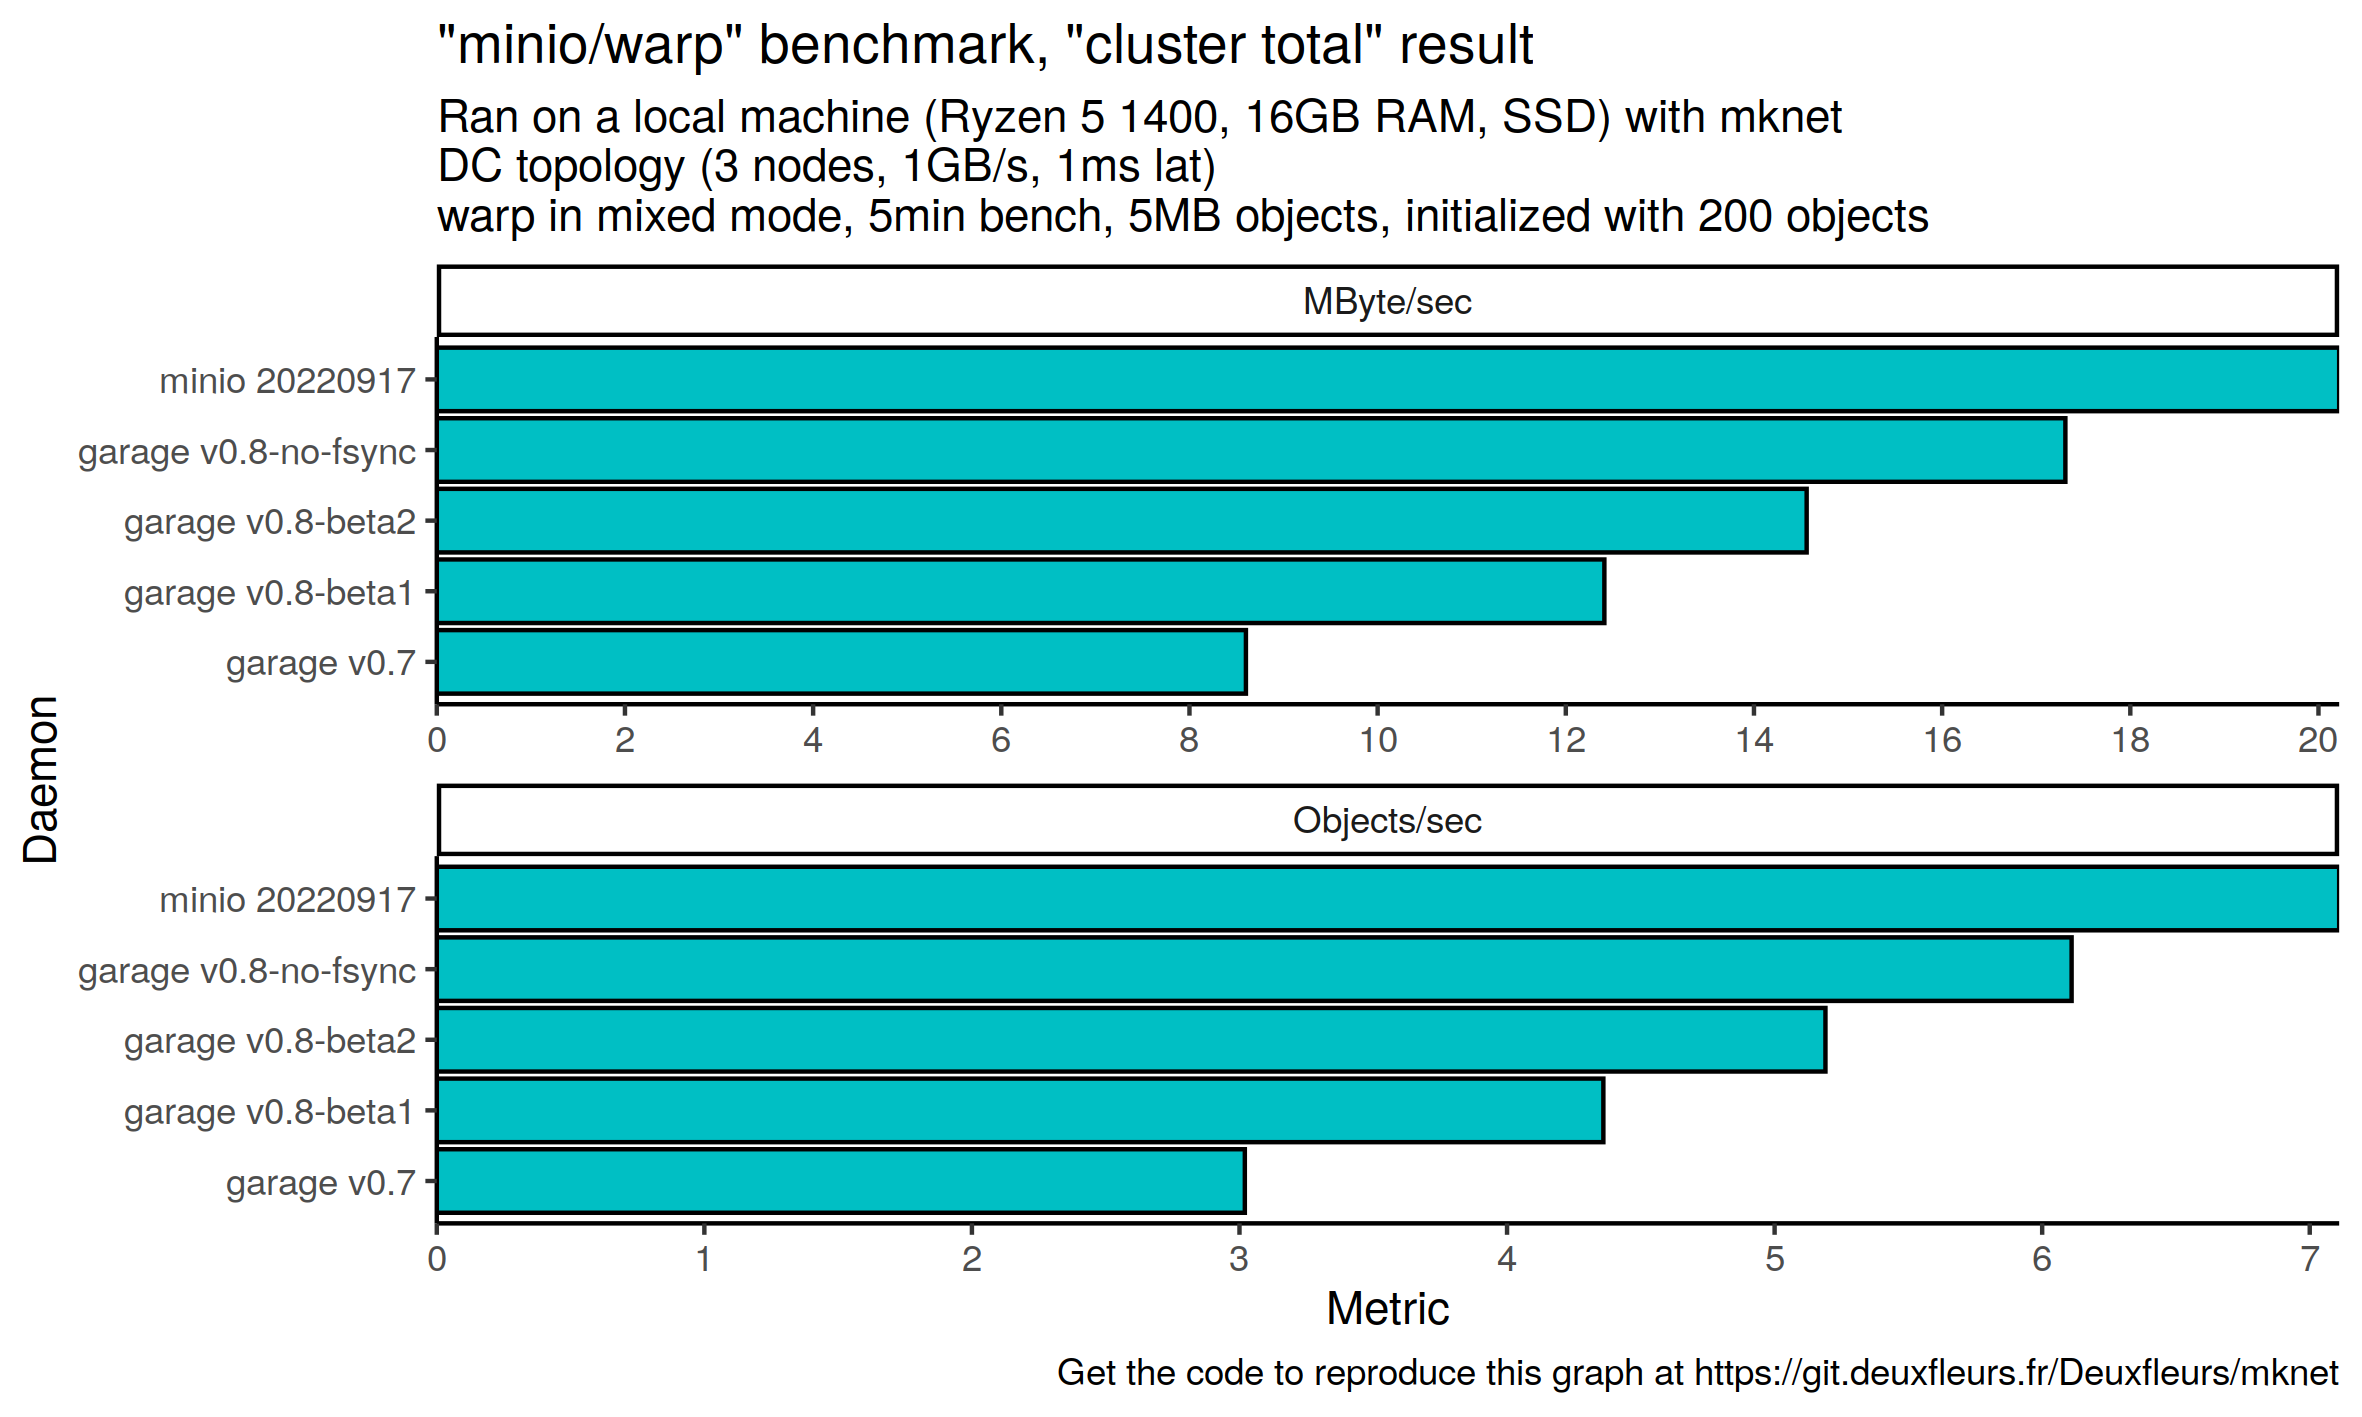
\includegraphics[width=.7\linewidth]{../assets/perf/io-0.7-0.8-minio.png}
	\end{center}
\end{frame}

% ====================== v0.9.0 ===============================

\begin{frame}
	\begin{center}
		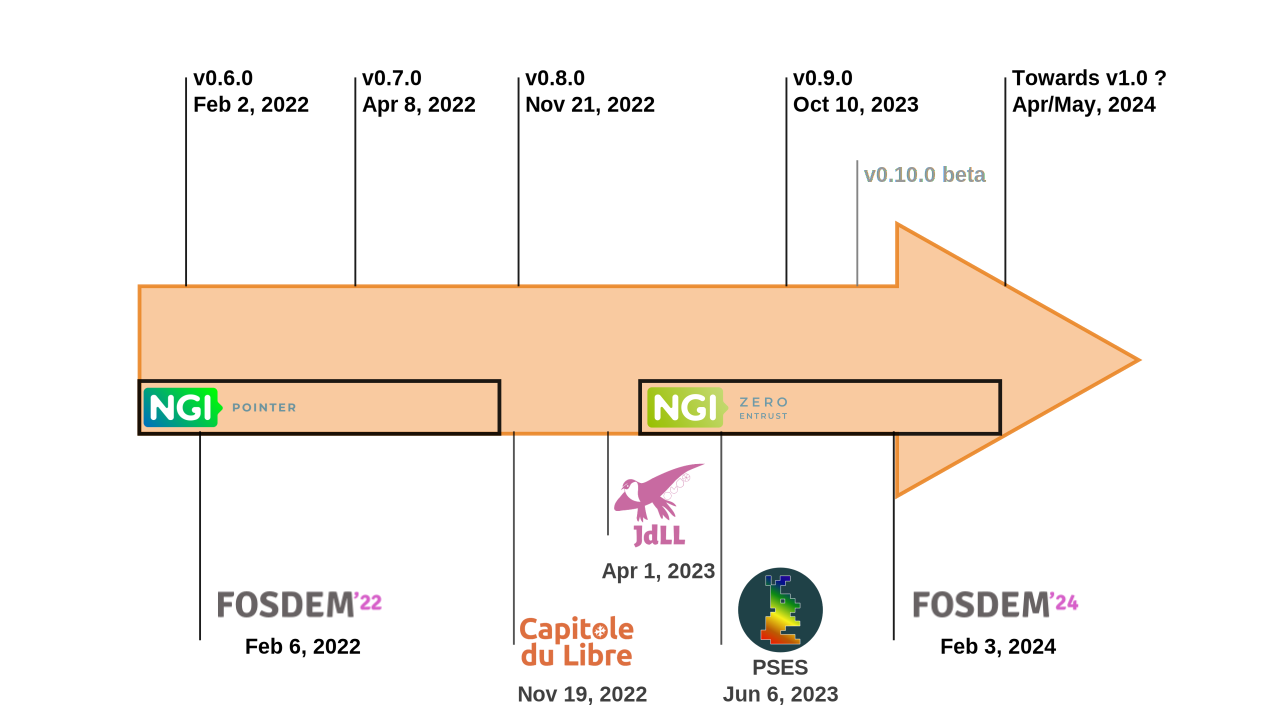
\includegraphics[width=.8\linewidth]{../assets/timeline-22-24.pdf}
	\end{center}
\end{frame}

\begin{frame}
	\frametitle{October 2023 - Garage v0.9.0}
	Focus on \underline{streamlining \& usability}
	\vspace{2em}
	\begin{itemize}
		\item Support multiple HDDs per node
			\vspace{1em}
		\item S3 compatibility: 
			\vspace{1em}
			\begin{itemize}
				\item support basic lifecycle configurations
					\vspace{.5em}
				\item allow for multipart upload part retries
			\end{itemize}
			\vspace{1em}
		\item LMDB by default, deprecation of Sled
			\vspace{1em}
		\item New layout computation algorithm
	\end{itemize}
\end{frame}


\begin{frame}
	\frametitle{Layout computation}
	\begin{overprint}
		\onslide<1>
		\begin{center}
			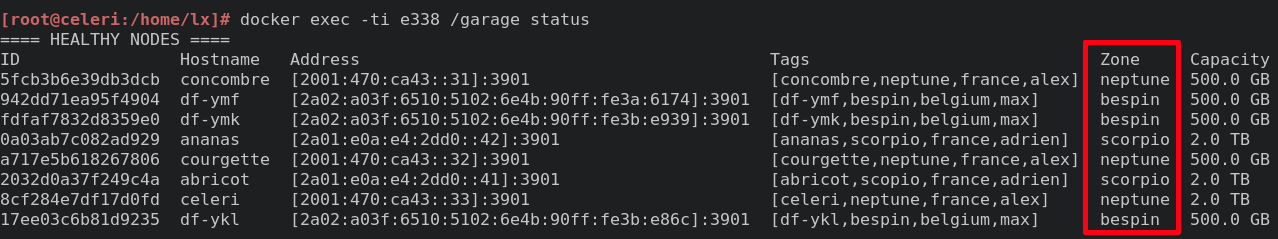
\includegraphics[width=\linewidth, trim=0 0 0 -4cm]{../assets/screenshots/garage_status_0.9_prod_zonehl.png}
		\end{center}
		\onslide<2>
		\begin{center}
			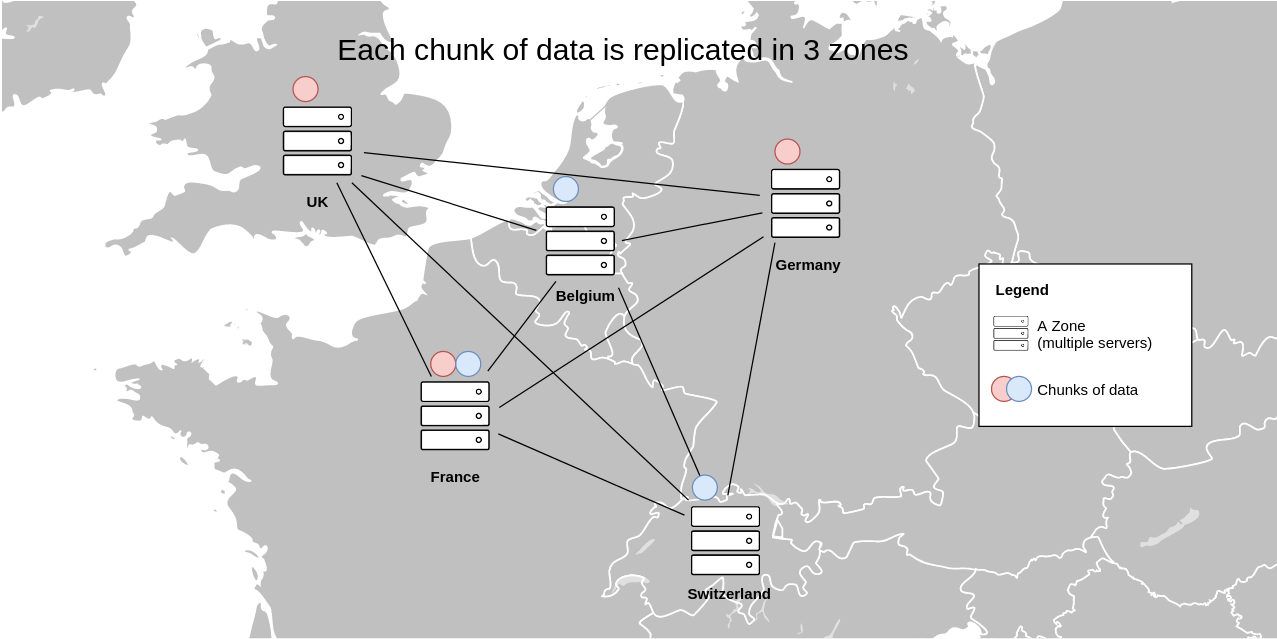
\includegraphics[width=.7\linewidth]{../assets/map.png}
		\end{center}
	\end{overprint}
	\vspace{1em}
	Garage stores replicas on different zones when possible
\end{frame}

\begin{frame}
	\frametitle{What a "layout" is}
		\textbf{A layout is a precomputed index table:}
		\vspace{1em}

		{\footnotesize
			\begin{center}
			\begin{tabular}{|l|l|l|l|}
				\hline
				\textbf{Partition} & \textbf{Node 1} & \textbf{Node 2} & \textbf{Node 3} \\
				\hline
				\hline
				Partition 0 & df-ymk (bespin) & Abricot (scorpio) & Courgette (neptune) \\
				\hline
				Partition 1 & Ananas (scorpio) & Courgette (neptune) & df-ykl (bespin) \\
				\hline
				Partition 2 & df-ymf (bespin) & Celeri (neptune) & Abricot (scorpio) \\
				\hline
				\hspace{1em}$\vdots$ & \hspace{1em}$\vdots$ & \hspace{1em}$\vdots$ & \hspace{1em}$\vdots$ \\
				\hline
				Partition 255 & Concombre (neptune) & df-ykl (bespin) & Abricot (scorpio) \\
				\hline
			\end{tabular}
			\end{center}
		}

	\vspace{2em}
	\visible<2->{
		The index table is built centrally using an optimal algorithm,\\
		then propagated to all nodes
	}

	\vspace{1em}
	\visible<3->{
		\footnotesize
		Oulamara, M., \& Auvolat, A. (2023). \emph{An algorithm for geo-distributed and redundant storage in Garage}.\\ arXiv preprint arXiv:2302.13798.
	}
\end{frame}



% ====================== v0.10.0 ===============================

\begin{frame}
	\begin{center}
		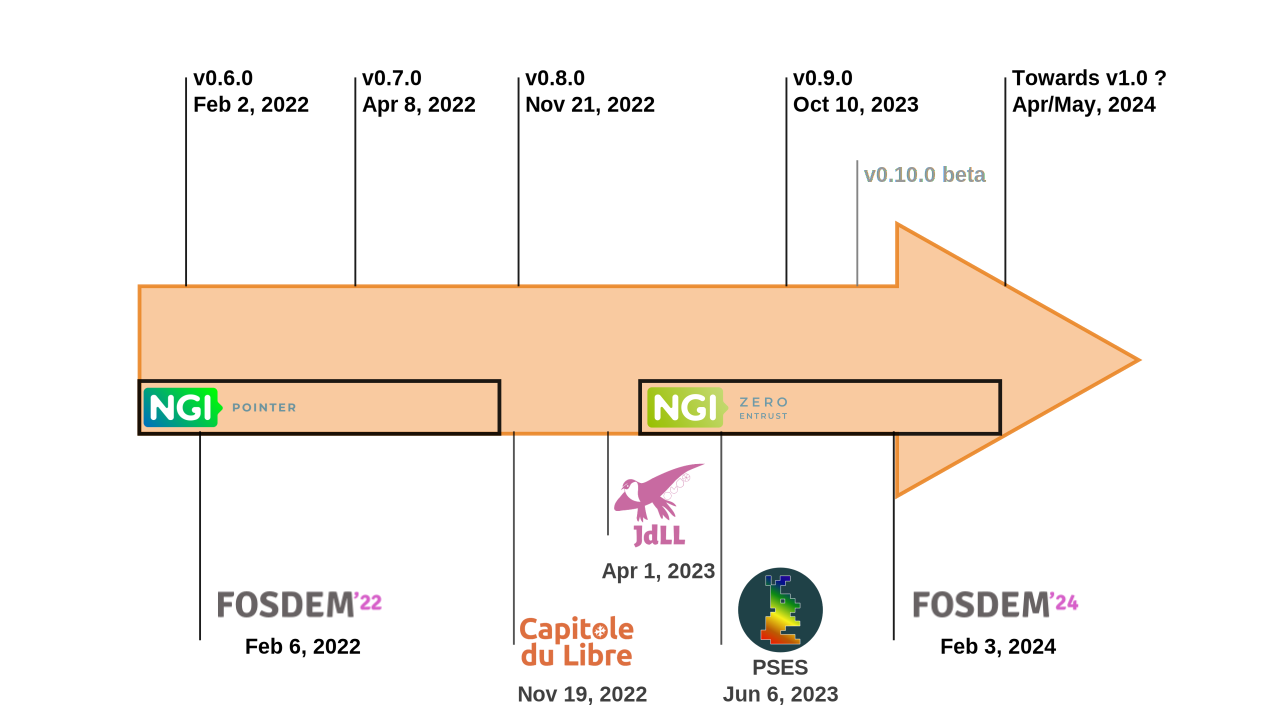
\includegraphics[width=.8\linewidth]{../assets/timeline-22-24.pdf}
	\end{center}
\end{frame}

\begin{frame}
	\frametitle{October 2023 - Garage v0.10.0 beta}
	Focus on \underline{consistency}
	\vspace{2em}
	\begin{itemize}
		\item Fix consistency issues when reshuffling data
	\end{itemize}
\end{frame}

\begin{frame}
	\frametitle{Working with weak consistency}
	Not using consensus limits us to the following:
	\vspace{2em}
	\begin{itemize}
		\item<2-> \textbf{Conflict-free replicated data types} (CRDT)\\
			\vspace{1em}
			{\footnotesize Non-transactional key-value stores such as S3 are equivalent to a simple CRDT:\\
			a map of \textbf{last-writer-wins registers} (each key is its own CRDT)}
			\vspace{1.5em}
		\item<3-> \textbf{Read-after-write consistency}\\
			\vspace{1em}
			{\footnotesize Can be implemented using quorums on read and write operations}
	\end{itemize}
\end{frame}

\begin{frame}[t]
	\frametitle{CRDT read-after-write consistency using quorums}

	\vspace{1em}
	{\small
		\textbf{Property:} If client 1 did an operation $write(x)$ and received an OK response,\\
			\hspace{2cm} and client 2 starts an operation $read()$ after client 1 received OK,\\
			\hspace{2cm} then client 2 will read a value $x' \sqsupseteq x$.
	}

	\vspace{1.5em}
	\begin{overprint}
		\onslide<2-9>
		\begin{figure}
			\centering
			\footnotesize
			\def\svgwidth{.7\textwidth}
			\only<2>{\import{../assets/lattice/}{lattice1.pdf_tex}}%
			\only<3>{\import{../assets/lattice/}{lattice2.pdf_tex}}%
			\only<4>{\import{../assets/lattice/}{lattice3.pdf_tex}}%
			\only<5>{\import{../assets/lattice/}{lattice4.pdf_tex}}%
			\only<6>{\import{../assets/lattice/}{lattice5.pdf_tex}}%
			\only<7>{\import{../assets/lattice/}{lattice6.pdf_tex}}%
			\only<8>{\import{../assets/lattice/}{lattice7.pdf_tex}}%
			\only<9>{\import{../assets/lattice/}{lattice8.pdf_tex}}%
		\end{figure}
		
		\onslide<10>
		\begin{minipage}{.10\textwidth}
			~
		\end{minipage}
		\begin{minipage}{.40\textwidth}
			\footnotesize
			\textbf{Algorithm $write(x)$:}
			\begin{enumerate}
				\item Broadcast $write(x)$ to all nodes
				\item Wait for $k > n/2$ nodes to reply OK
				\item Return OK
			\end{enumerate}
		\end{minipage}
		\begin{minipage}{.40\textwidth}
			\footnotesize
			\vspace{1em}
			\textbf{Algorithm $read()$:}
			\begin{enumerate}
				\item Broadcast $read()$ to all nodes
				\item Wait for $k > n/2$ nodes to reply\\
					with values $x_1, \dots, x_k$
				\item Return $x_1 \sqcup \dots \sqcup x_k$
			\end{enumerate}
		\end{minipage}
	\end{overprint}
\end{frame}

\begin{frame}
	\frametitle{A hard problem: layout changes}
	\begin{itemize}
		\item We rely on quorums $k > n/2$ within each partition:\\
			$$n=3,~~~~~~~k\ge 2$$
		\item<2-> When rebalancing, the set of nodes responsible for a partition can change:\\

			\vspace{1em}
			\begin{minipage}{.04\linewidth}~
			\end{minipage}
			\begin{minipage}{.40\linewidth}
			{\tiny
				\begin{tabular}{|l|l|l|l|}
					\hline
					\textbf{Partition} & \textbf{Node 1} & \textbf{Node 2} & \textbf{Node 3} \\
					\hline
					\hline
					Partition 0 & \textcolor{Crimson}{df-ymk}  & Abricot  & \textcolor{Crimson}{Courgette} \\
					\hline
					Partition 1 & Ananas  & \textcolor{Crimson}{Courgette} & \textcolor{Crimson}{df-ykl}  \\
					\hline
					Partition 2 & \textcolor{Crimson}{df-ymf}  & \textcolor{Crimson}{Celeri} & Abricot  \\
					\hline
					\hspace{1em}$\dots$ & \hspace{1em}$\dots$ & \hspace{1em}$\dots$ & \hspace{1em}$\dots$ \\
					\hline
				\end{tabular}
			}
			\end{minipage}
			\begin{minipage}{.04\linewidth}
				$\to$
			\end{minipage}
			\begin{minipage}{.40\linewidth}
			{\tiny
				\begin{tabular}{|l|l|l|l|}
					\hline
					\textbf{Partition} & \textbf{Node 1} & \textbf{Node 2} & \textbf{Node 3} \\
					\hline
					\hline
					Partition 0 & \textcolor{ForestGreen}{Dahlia}  & Abricot  & \textcolor{ForestGreen}{Eucalyptus} \\
					\hline
					Partition 1 & Ananas  & \textcolor{ForestGreen}{Euphorbe}  & \textcolor{ForestGreen}{Doradille} \\
					\hline
					Partition 2 & \textcolor{ForestGreen}{Dahlia}  & \textcolor{ForestGreen}{Echinops} & Abricot  \\
					\hline
					\hspace{1em}$\dots$ & \hspace{1em}$\dots$ & \hspace{1em}$\dots$ & \hspace{1em}$\dots$ \\
					\hline
				\end{tabular}
			}
			\end{minipage}

			\vspace{2em}
		\item<3-> During the rebalancing, new nodes don't yet have the data,\\
			~~~~~~~~~~~~~~~~~~~and old nodes want to get rid of the data to free up space\\
			\vspace{1.2em}
			$\to$ risk of inconsistency, \textbf{how to coordinate?}
	\end{itemize}
\end{frame}

\begin{frame}
	\frametitle{Handling layout changes without losing consistency}
	\begin{minipage}{.55\textwidth}
		\begin{itemize}
			\item \textbf{Solution:}\\
				\vspace{.5em}
				\begin{itemize}
					\item keep track of data transfer to new nodes
						\vspace{.5em}
					\item use multiple write quorums\\
						(new nodes + old nodes\\
						while data transfer is in progress)
						\vspace{.5em}
					\item switching reads to new nodes\\
						only once copy is finished
				\end{itemize}
				\vspace{1em}
			\item \textbf{Implemented} in v0.10
				\vspace{1em}
			\item \textbf{Validated} with Jepsen testing
		\end{itemize}
	\end{minipage}
	\begin{minipage}{.23\textwidth}
		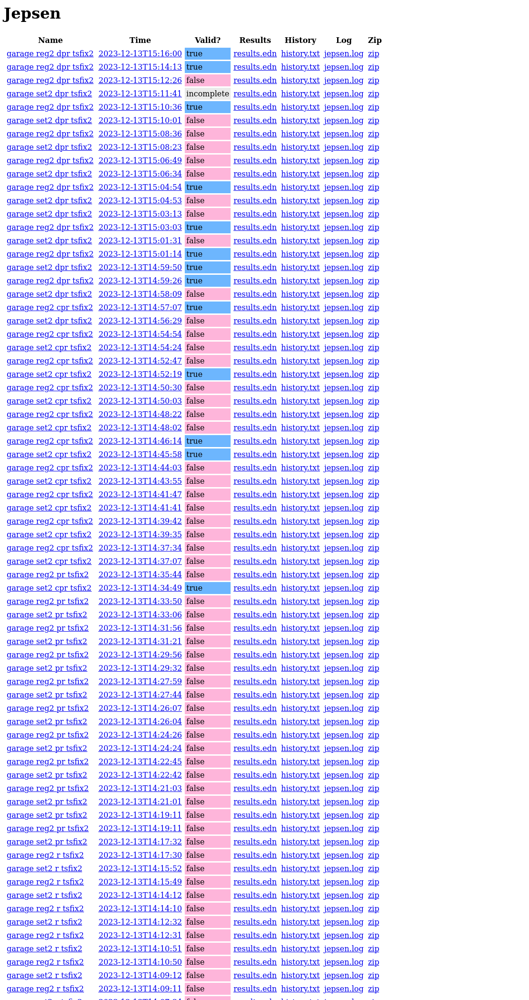
\includegraphics[width=3cm]{../assets/jepsen-0.9.png}\\
		{\footnotesize Garage v0.9.0}
	\end{minipage}
	\begin{minipage}{.2\textwidth}
		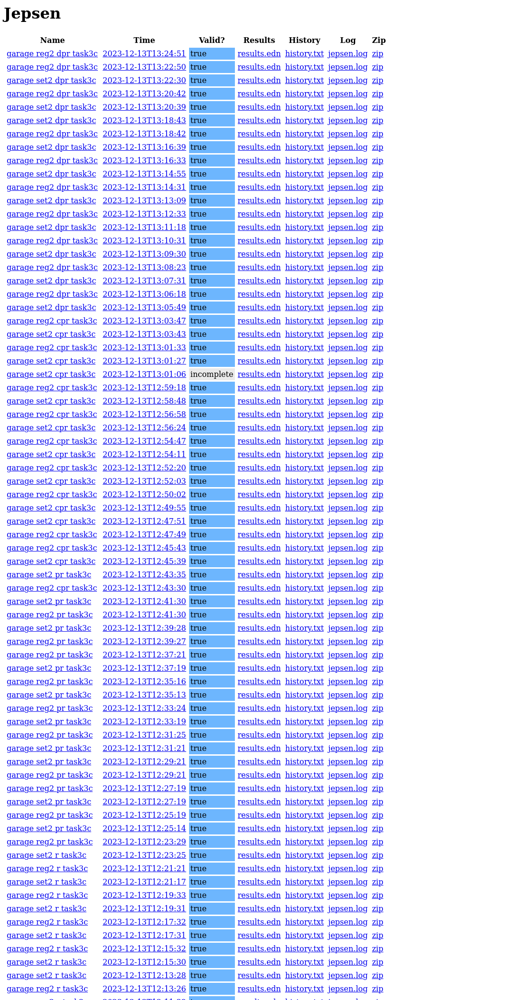
\includegraphics[width=3cm]{../assets/jepsen-0.10.png}\\
		{\footnotesize Garage v0.10 beta}
	\end{minipage}
\end{frame}

% ====================== v0.10.0 ===============================

\begin{frame}
	\begin{center}
		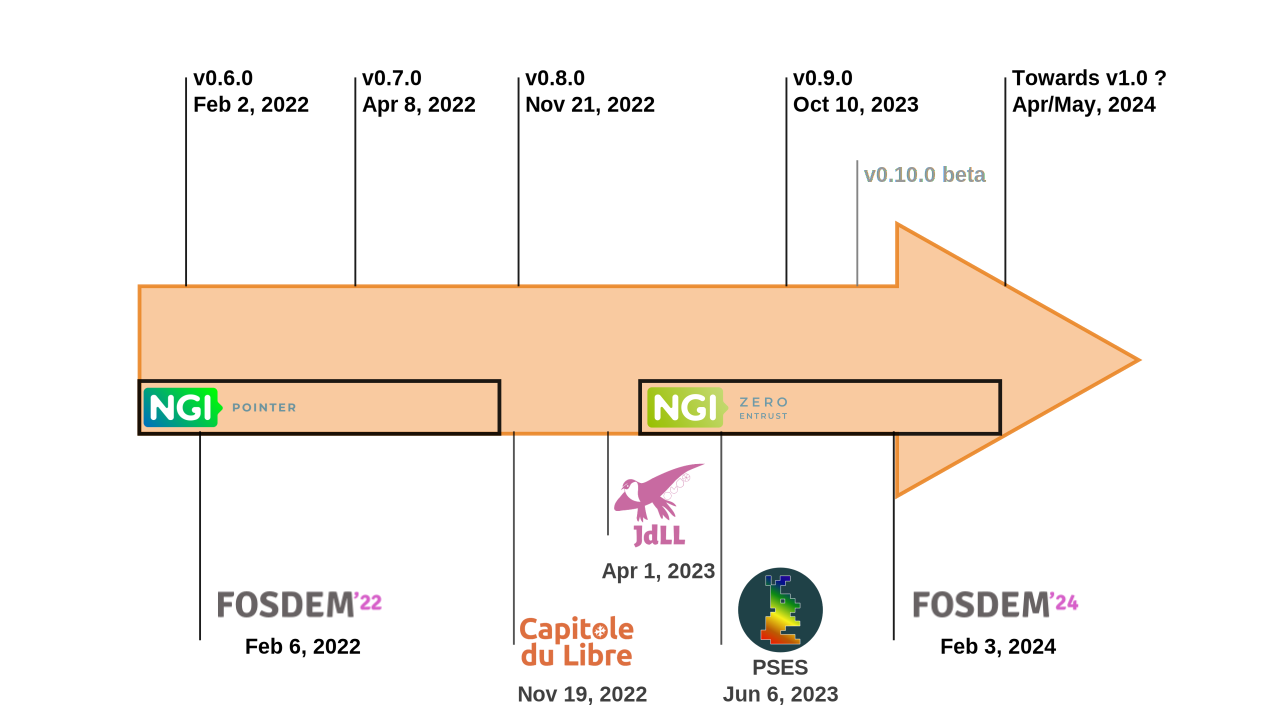
\includegraphics[width=.8\linewidth]{../assets/timeline-22-24.pdf}
	\end{center}
\end{frame}

\begin{frame}
	\frametitle{Towards v1.0...}
	Focus on \underline{security \& stability}
	\vspace{2em}
	\begin{itemize}
		\item \textbf{Security audit} in progress by Radically Open Security
			\vspace{1em}
		\item Misc. S3 features (SSE-C, ...) and compatibility fixes
			\vspace{1em}
		\item Improve UX
			\vspace{1em}
		\item Fix bugs
	\end{itemize}
\end{frame}

\begin{frame}
	\frametitle{...and beyond!}
	\begin{center}
		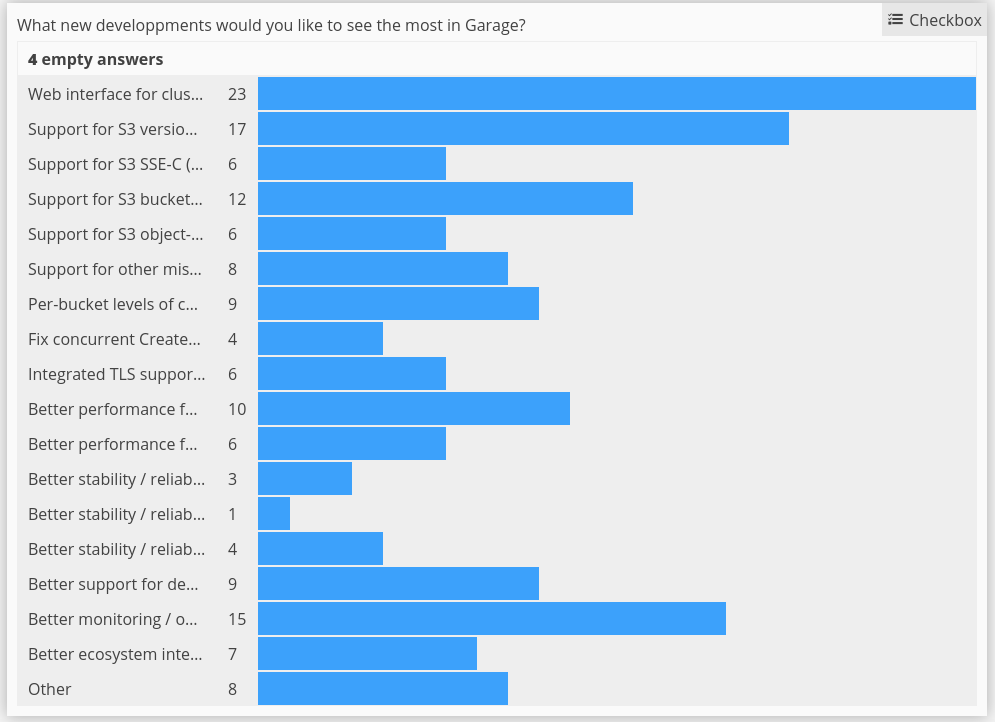
\includegraphics[width=.6\linewidth]{../assets/survey_requested_features.png}
	\end{center}
\end{frame}

% ======================================== OPERATING
% ======================================== OPERATING
% ======================================== OPERATING


\section{Operating big Garage clusters}

\begin{frame}
	\frametitle{Operating Garage}
	\begin{center}
		\only<1-2>{
			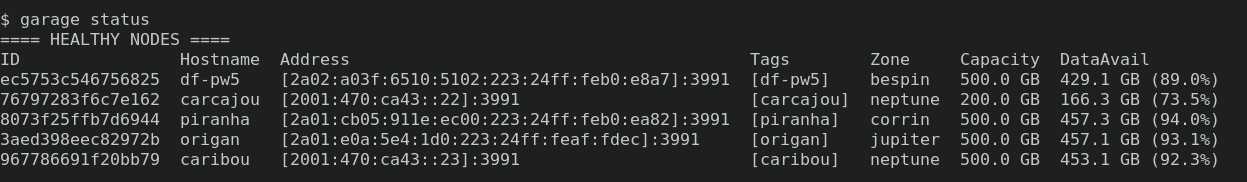
\includegraphics[width=.9\linewidth]{../assets/screenshots/garage_status_0.10.png}
			\\\vspace{1em}
			\visible<2>{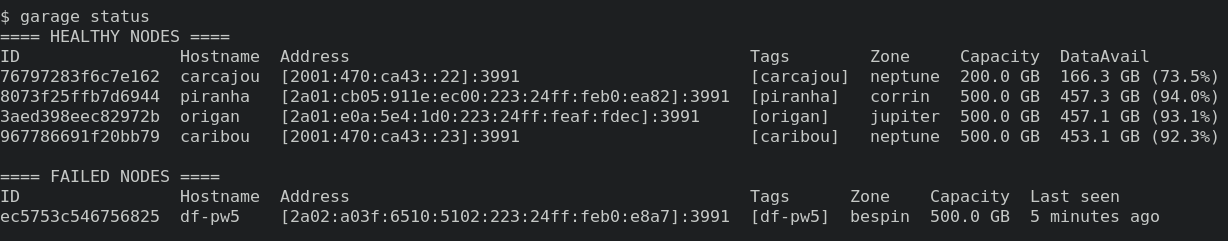
\includegraphics[width=.9\linewidth]{../assets/screenshots/garage_status_unhealthy_0.10.png}}
		}
	\end{center}
\end{frame}

\begin{frame}
	\frametitle{Garage's architecture}
	\begin{center}
		\only<1>{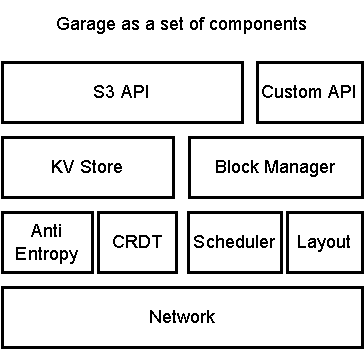
\includegraphics[width=.45\linewidth]{../assets/garage.drawio.pdf}}%
		\only<2>{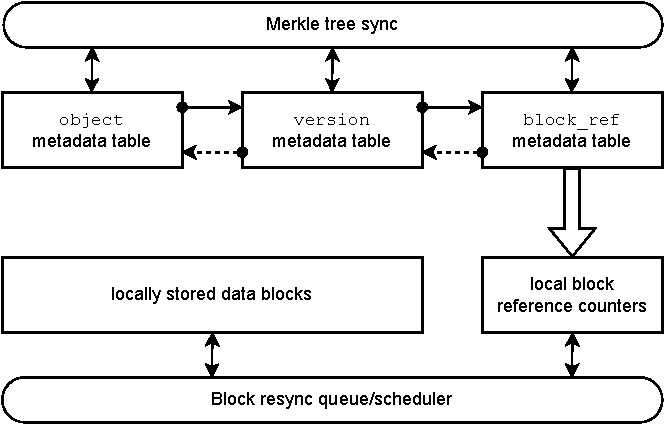
\includegraphics[width=.6\linewidth]{../assets/garage_sync.drawio.pdf}}%
	\end{center}
\end{frame}

\begin{frame}
	\frametitle{Digging deeper}
	\begin{center}
		\only<1>{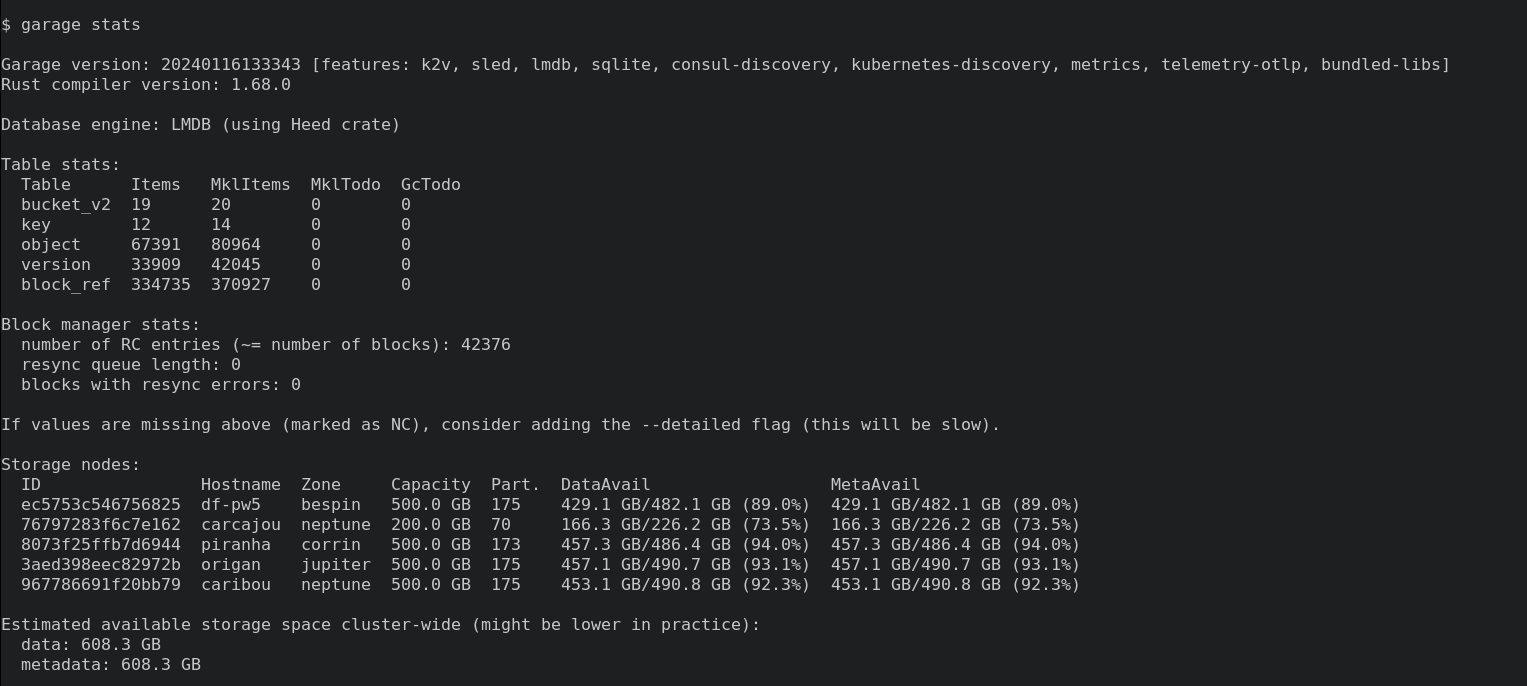
\includegraphics[width=.9\linewidth]{../assets/screenshots/garage_stats_0.10.png}}
		\only<2>{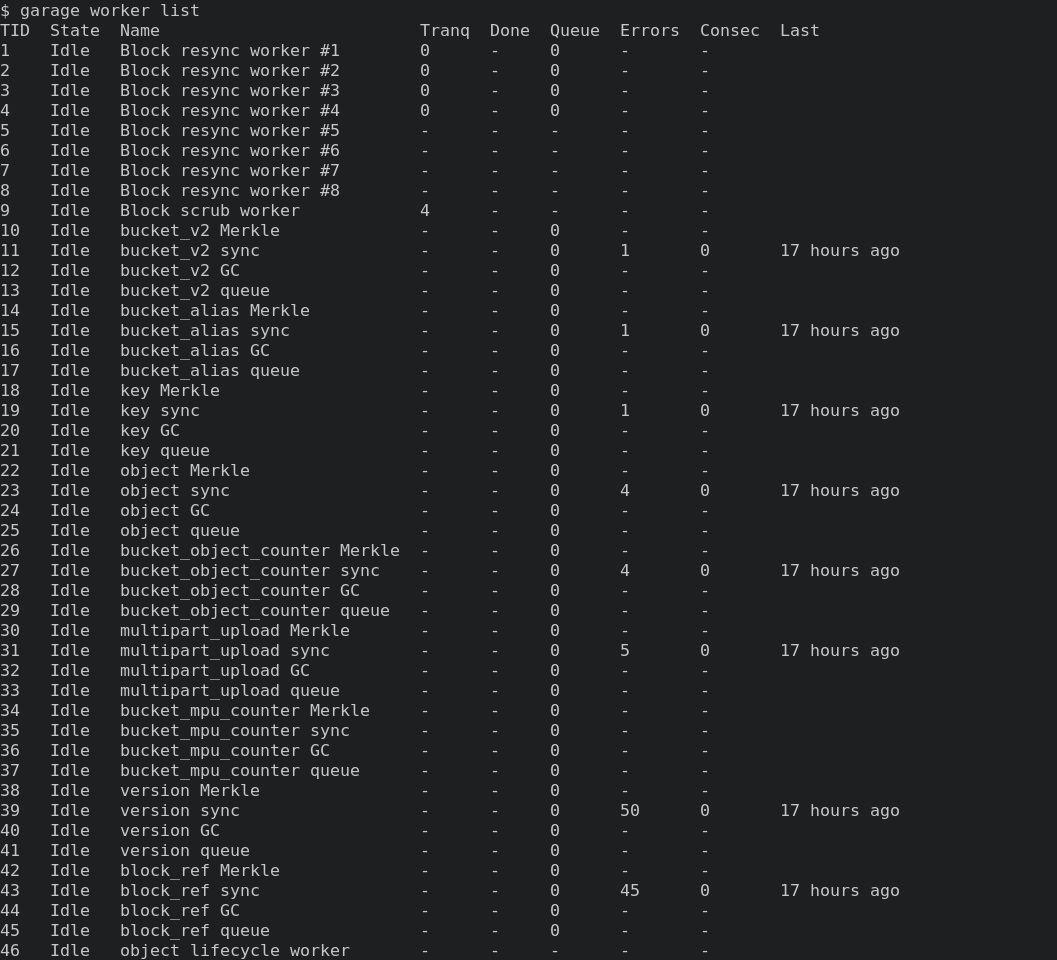
\includegraphics[width=.5\linewidth]{../assets/screenshots/garage_worker_list_0.10.png}}
		\only<3>{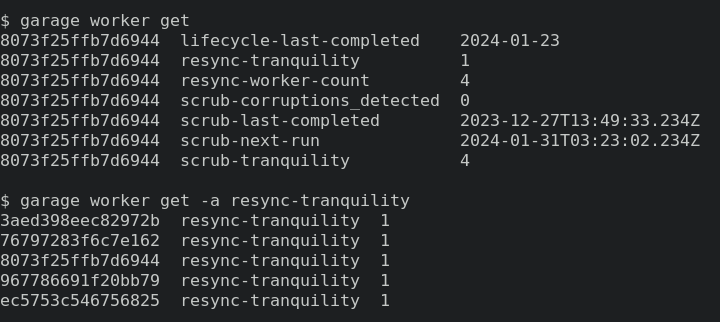
\includegraphics[width=.6\linewidth]{../assets/screenshots/garage_worker_param_0.10.png}}
	\end{center}
\end{frame}

\begin{frame}
	\frametitle{Potential limitations and bottlenecks}
	\begin{itemize}
		\item Global:
			\begin{itemize}
				\item Max. $\sim$100 nodes per cluster (excluding gateways)
			\end{itemize}
			\vspace{1em}
		\item Metadata:
			\begin{itemize}
				\item One big bucket = bottleneck, object list on 3 nodes only
			\end{itemize}
			\vspace{1em}
		\item Block manager:
			\begin{itemize}
				\item Lots of small files on disk
				\item Processing the resync queue can be slow
			\end{itemize}
	\end{itemize}
\end{frame}

\begin{frame}
	\frametitle{Deployment advice for very large clusters}
	\begin{itemize}
		\item Metadata storage:
			\begin{itemize}
				\item ZFS mirror (x2) on fast NVMe
				\item Use LMDB storage engine
			\end{itemize}
			\vspace{.5em}
		\item Data block storage:
			\begin{itemize}
				\item Use Garage's native multi-HDD support
				\item XFS on individual drives
				\item Increase block size (1MB $\to$ 10MB, requires more RAM and good networking)
				\item Tune \texttt{resync-tranquility} and \texttt{resync-worker-count} dynamically
			\end{itemize}
			\vspace{.5em}
		\item Other :
			\begin{itemize}
				\item Split data over several buckets
				\item Use less than 100 storage nodes
				\item Use gateway nodes
			\end{itemize}
			\vspace{.5em}
	\end{itemize}
	Our deployments: $< 10$ TB. Some people have done more!
\end{frame}


% ======================================== END
% ======================================== END
% ======================================== END

\begin{frame}
	\frametitle{Where to find us}
	\begin{center}
			\includegraphics[width=.25\linewidth]{../../logo/garage_hires.png}\\
			\vspace{-1em}
		\url{https://garagehq.deuxfleurs.fr/}\\
		\url{mailto:garagehq@deuxfleurs.fr}\\
		\texttt{\#garage:deuxfleurs.fr} on Matrix

		\vspace{1.5em}
			
\includegraphics[width=.06\linewidth]{../assets/logos/rust_logo.png}
			
\includegraphics[width=.13\linewidth]{../assets/logos/AGPLv3_Logo.png}
	\end{center}
\end{frame}

\end{document}

%% vim: set ts=4 sw=4 tw=0 noet spelllang=en :
